% Author-approved topology framing; bounded revision intent is recorded separately.
% Preserve the original and dated revision-intent manifests alongside this source.
% Archival and completed fresh numerical bindings are checked separately.
% The bibliography is inline; the topology figure is a local project asset.
\RequirePackage{fix-cm}
\documentclass[11pt,letterpaper]{article}
\usepackage[utf8]{inputenc}
\usepackage[T1]{fontenc}
\usepackage[margin=1in]{geometry}
\usepackage{amsmath,amssymb}
\usepackage{booktabs,array,tabularx,ragged2e}
\usepackage{graphicx}
\usepackage{fontawesome5}
\usepackage{placeins}
\usepackage{xcolor}
\usepackage{microtype}
\usepackage{url}
\definecolor{paperblue}{HTML}{3456CC}
\usepackage[colorlinks=true,linkcolor=paperblue,citecolor=paperblue,urlcolor=paperblue,
  pdftitle={Depth-Read Sharing in Grouped-Query Attention},
  pdfauthor={Zimu Zhao}]{hyperref}
\newcolumntype{Y}{>{\RaggedRight\arraybackslash}X}
\setlength{\parindent}{0pt}
\setlength{\parskip}{0.65em}
\setlength{\emergencystretch}{2em}
\newcommand{\paperTitleStyle}{\fontsize{13.8pt}{15.8pt}\selectfont\bfseries}
\newcommand{\frontMatterTitleStyle}{\fontsize{15.15pt}{17.2pt}\selectfont\bfseries}
\newcommand{\route}[1]{\textsf{#1}}
\newcommand{\Loss}{\mathcal{L}}
\newcommand{\pending}[1]{\textcolor{paperblue}{\textit{Draft status: #1}}}

% Rounded display values; full precision and extraction paths are in source-ledger.json.
\newcommand{\LossAAAA}{4.137027}
\newcommand{\LossABAA}{4.133390}
\newcommand{\LossAABA}{4.102798}
\newcommand{\LossAAAB}{4.078685}
\newcommand{\LossAABB}{4.123400}
\newcommand{\LossABBA}{4.093913}
\newcommand{\LossAABC}{4.076407}
\newcommand{\LossABBC}{4.073389}
\newcommand{\DeltaABAA}{-0.003636}
\newcommand{\LowABAA}{-0.005233}
\newcommand{\HighABAA}{-0.002051}
\newcommand{\DeltaABBC}{-0.005296}
\newcommand{\LowABBC}{-0.008065}
\newcommand{\HighABBC}{-0.002988}
\newcommand{\FamilyLowABBC}{-0.008507}
\newcommand{\FamilyHighABBC}{-0.002715}
\newcommand{\DeltaSameCount}{-0.003018}
\newcommand{\LowSameCount}{-0.004925}
\newcommand{\HighSameCount}{-0.001230}
\newcommand{\DeltaLocal}{0.028681}
\newcommand{\LowLocal}{0.026421}
\newcommand{\HighLocal}{0.030987}
\newcommand{\RatioStep}{1.140}
\newcommand{\RatioPrefill}{1.322}
\newcommand{\RatioDecode}{1.683}
\newcommand{\CachePrefill}{90}
\newcommand{\CacheDecode}{101.25}
% Completed three-seed evidence; never pooled with the archival macros above.
\newcommand{\FreshPrimaryMean}{-0.000169}
\newcommand{\FreshPrimarySD}{0.007516}
\newcommand{\FreshAllocationMean}{0.002532}
\newcommand{\FreshAllocationSD}{0.013596}
\newcommand{\StageAPrimaryMean}{-0.068322}
\newcommand{\StageAPrimarySD}{0.012519}
\newcommand{\StageAAABCMean}{-0.070815}
\newcommand{\StageAABBCMean}{-0.067302}


% Completed two-read study / common-artifact claim bindings.
\newcommand{\TwoReadWeakGain}{0.007977}
\newcommand{\TwoReadStrongGain}{0.068322}
\newcommand{\TwoReadGainRatio}{8.57}
\newcommand{\KVGroupedMean}{-0.036192}
\newcommand{\FollowABBCvsAAAB}{0.001020}
\newcommand{\FollowABBCvsAABC}{0.003513}
\newcommand{\FollowAABCvsAAAB}{-0.002493}
\newcommand{\AABCSeedReversal}{0.009271}
\newcommand{\LastLRPercent}{99.39}
% Post-result descriptive comparison within one driver; not a promotion test.
\newcommand{\WithinDriverMean}{-0.045051}
\newcommand{\WithinDriverSD}{0.006573}
\newcommand{\WithinDriverSeedFirst}{-0.047026}
\newcommand{\WithinDriverSeedSecond}{-0.037718}
\newcommand{\WithinDriverSeedThird}{-0.050410}

% Post-result, token-averaged native routing-weight distances; no seed test.
\newcommand{\ProfileAAABHalfLone}{0.2283}
\newcommand{\ProfileABBCHalfAB}{0.0862}
\newcommand{\ProfileABBCHalfAC}{0.2148}
\newcommand{\ProfileABBCHalfBC}{0.2268}

% Selected archival controls; each value retains its own parent and artifact.
\newcommand{\ArchiveHardQKV}{0.286143}
\newcommand{\ArchiveHardQKVLow}{0.275798}
\newcommand{\ArchiveHardQKVHigh}{0.296909}
\newcommand{\ArchiveLocalQ}{0.054053}
\newcommand{\ArchiveLocalQLow}{0.051504}
\newcommand{\ArchiveLocalQHigh}{0.056699}
\newcommand{\ArchiveHybridQ}{-0.000671}
\newcommand{\ArchiveHybridQLow}{-0.002908}
\newcommand{\ArchiveHybridQHigh}{0.001551}
\newcommand{\ArchiveSoftBoth}{0.008978}
\newcommand{\ArchiveSoftBothLow}{0.006670}
\newcommand{\ArchiveSoftBothHigh}{0.011313}
\newcommand{\ArchiveSoftOne}{0.004125}
\newcommand{\ArchiveSoftOneLow}{0.002006}
\newcommand{\ArchiveSoftOneHigh}{0.006325}
\newcommand{\ArchiveSeparate}{-0.001915}
\newcommand{\ArchiveSeparateLow}{-0.003664}
\newcommand{\ArchiveSeparateHigh}{-0.000191}
\newcommand{\ArchiveCollapse}{0.059498}
\newcommand{\ArchiveRequest}{0.001558}
\newcommand{\ArchiveRequestLow}{-0.000137}
\newcommand{\ArchiveRequestHigh}{0.003277}
\newcommand{\ArchiveContrast}{0.001734}
\newcommand{\ArchiveContrastLow}{0.000019}
\newcommand{\ArchiveContrastHigh}{0.003420}

\author{Zimu Zhao}
\begin{document}
\begin{center}
  \rule{\textwidth}{1.8pt}\par
  \vspace{0.9em}
  {\paperTitleStyle Depth-Read Sharing in Grouped-Query Attention\par}
  \vspace{0.9em}
  \rule{\textwidth}{1.8pt}\par
  \vspace{0.5em}
  {\textbf{Zimu Zhao}\quad\href{mailto:zimmer061310@gmail.com}{\textcolor{black}{zimmer061310@gmail.com}}\par}
  {\faGithub\,\href{https://github.com/Zimmer061310/Depth-Read-Sharing-in-Grouped-Query-Attention}{\texttt{Depth-Read-Sharing-in-Grouped-Query-Attention}}\par}
\end{center}

\begin{center}
  {\frontMatterTitleStyle Abstract}
\end{center}
Depth routing lets attention projections read mixtures of earlier branch
outputs. We study which consumers within a grouped-query attention (GQA)
group should share a read under Multi-Head Attention Residuals (MHAR).
Holding GQA and full-width feature access fixed, we train eight patterns
over $(Q_1,Q_2,K,V)$ with three matched seeds at approximately 1.08B parameters,
giving 24 models. All seven multi-read patterns have lower loss than shared-read
MHAR in every seed on a common frozen evaluation. All five two-read patterns
meet their predeclared practical rule, with mean reductions from
\TwoReadWeakGain{} to \TwoReadStrongGain{} nats/target. Four let $V$ share its read;
their parent comparisons are cross-driver, and early parity at update 101
does not establish endpoint driver equivalence. Among these four patterns,
driver and read count match, yet the same loss ordering holds in every seed.
Neither three-read pattern improves on the value-separated two-read control
in every seed, and the selected refinement fails both predeclared criteria.
All runs stop at 2,000 updates of a 20,000-update schedule, with learning rate
still \LastLRPercent{}\% of peak. The evidence supports studying sharing assignment
alongside read count; persistence and equal-compute benefit remain unmeasured.

\section{Introduction}
\label{sec:intro}
Attention Residuals replaces fixed residual accumulation with a learned
mixture of earlier layer outputs~\cite{attnres2026}. % <!--ref:attnres2026--><!--anchor:section:3.1-->
MHAR lets different feature slices use different depth
mixtures~\cite{mhar2026}. % <!--ref:mhar2026--><!--anchor:section:2.3-->
These methods determine how a layer reads its history. A separate question
is which attention projections should share that read.

GQA gives each query group a shared key and value
head~\cite{gqa2023}. % <!--ref:gqa2023--><!--anchor:abstract-->
MHAR supplies feature-wise mixtures of residual depth to the attention
projections; GQA uses their queries, keys and values to attend across token
positions.
This head-sharing rule does not require the query, key and value projections
to receive the same input state. RD-AttnRes exploits this distinction by
using one depth read for queries and keys and another for
values~\cite{rd2026}. % <!--ref:rd2026--><!--anchor:section:3-->
We study alternative sharing patterns under a common MHAR parent:
\emph{which consumers within a GQA group should share a depth read?}
The GQA relationship and the depth-read operator stay fixed. With two query
heads per shared KV pair, the consumers are $(Q_1,Q_2,K,V)$.

We use MHAR to ask whether these consumers should share a read even when
depth retrieval is already feature-adaptive. MHAR determines how individual
feature subspaces retrieve residual history; the sharing pattern determines
which GQA consumers reuse the assembled full-width reads. Holding the MHAR
reader fixed lets us compare consumer assignments within this setting.

We encode a pattern by four letters for $(Q_1,Q_2,K,V)$.
Equal letters mean a shared read. Thus \route{AAAA} uses one read,
\route{AAAB} separates $V$, and \route{ABBC} separates one query while
keeping the other with $K$. The three-read control \route{AABC} keeps the
two queries together and separates $K$ and $V$. After read relabeling and
query-slot exchange, the space has 11 classes. We evaluate eight: the
shared-read parent, all five two-read classes, and two three-read patterns.
The parameter permutation
required for query-slot exchange and the untested classes are specified in
Appendix~\ref{app:model}.

The study separates three comparisons: multiple versus one read, assignment
at fixed read count, and the incremental benefit of a third read.
Every tested multi-read pattern has lower endpoint loss than the shared-read
parent in each seed, including assignments without singleton $V$.
Assignments differ substantially even when count and driver match.
The selected three-read \route{ABBC} does not meet its fresh improvement
criteria against either \route{AAAB} or \route{AABC}. Our contribution is the within-GQA sharing
formulation and its controlled empirical comparison, bounded by the driver
and training-horizon limits. Consumer-specific depth access, including
head-specific routing, is established prior
work~\cite{dca2025,dagformer2026}. % <!--ref:dca2025--><!--anchor:section:3.2--><!--ref:dagformer2026--><!--anchor:section:2.3-->
We examine which consumers benefit from sharing it.

\section{Depth-Read Sharing}
\label{sec:method}
At each attention site, MHAR reads the token embedding and preceding
attention/MLP branch outputs. Its eight feature-routing heads mix the source
slices independently and concatenate them into a full-width state. We
construct $R$ such states with independently trainable routing queries.
Within a site, all reads use the same source history and normalization parameters.
The MLP and final readout keep their native single reads.
The assignment is fixed across layers and GQA groups, while the connected
depth mixtures are learned and input-dependent. Feature-routing heads and
GQA groups are separate axes.

Let $\rho$ assign a read letter to each consumer. Suppressing layer and
token indices, the attention inputs are
\begin{align}
 h^r &= \operatorname{MHAR}(\mathcal S;q^r),
 &x^r&=\mathcal N_{\mathrm{in}}(h^r),\\
 \widetilde Q_{g,j}&=W^Q_{g,j}x^{\rho(Q_j)},\quad j\in\{1,2\},\\
 \widetilde K_g&=W^K_gx^{\rho(K)},
 &V_g&=W^V_gx^{\rho(V)}.
 \label{eq:sharing-inputs}
\end{align}
Here $\mathcal N_{\mathrm{in}}$ is the shared input RMSNorm~\cite{rmsnorm2019}. % <!--ref:rmsnorm2019--><!--anchor:abstract-->
Queries and keys receive the native head normalization, followed by
rotary position embeddings (RoPE)~\cite{roformer2024}. % <!--ref:roformer2024--><!--anchor:abstract-->
Both query heads still attend to the same $K_g,V_g$.
The $R$ full-width reads are constructed once per site and reused across
GQA groups. They do not create separate residual histories or KV caches.
Every projection retains full-width feature access.
Earlier feature-access controls test a different axis: restricting the
coordinates visible to a projection. We retain these controls and their
negative findings in Appendix~\ref{app:historical-controls}; they do not
establish that MHAR is necessary for consumer-sharing effects.
Appendix~\ref{app:model} gives the full operator and head layout.
Figure~\ref{fig:method} illustrates the computation and representative assignments.

\begin{figure}[!ht]
\centering
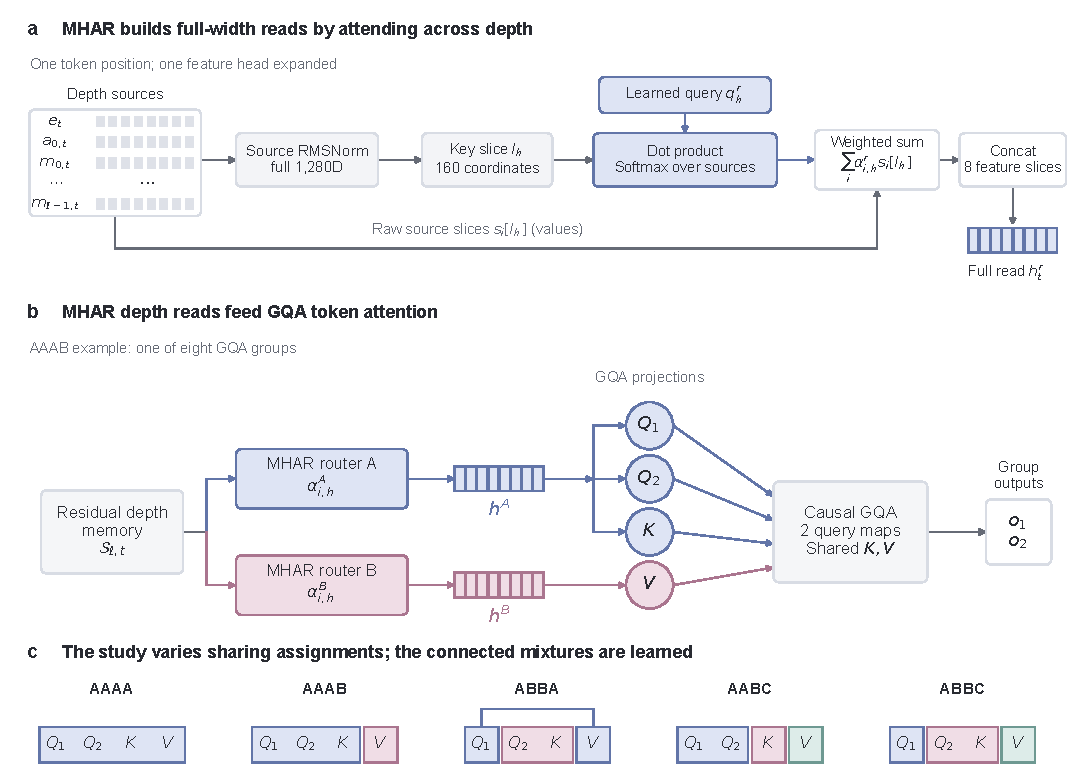
\includegraphics[width=\textwidth]{figures/consumer-sharing-method.pdf}
\caption{The MHAR--GQA computation and its sharing interface.
(a) At a fixed token position, source RMSNorm acts over the full model width
before selecting a feature slice. A learned pseudo-query produces a softmax
over depth sources; the mixture uses \emph{raw} source slices through the
value bypass. Concatenating eight 160-coordinate mixtures gives one
1,280-coordinate read. The operation repeats for each read and token
position; reads share the site's source bank and source-normalization
scales. The illustrated history is for $\ell>0$; layer 0 reads only the embedding.
(b) Worked \route{AAAB}: $A$ supplies $Q_1,Q_2,K$ and $B$ supplies $V$.
The input RMSNorm scales are shared between reads. Q/K head normalization
and RoPE precede two causal token-attention maps using one common KV pair;
$V$ receives neither head normalization nor RoPE. Native concatenation
collects all eight groups, retaining the physical $Q_2,Q_1$ order within
each group, before the output projection. The lower strip shows subsequent
source appends and the unchanged single-read MLP.
(c) Compact sharing examples; merged boxes identify a common read and the
connector joins non-adjacent members. The assignment is fixed; its mixtures
are learned and input-dependent. MHAR feature heads and GQA groups are
distinct axes. Colors name reads locally to each pattern; this schematic
shows no measured weights or separate residual histories.}
\label{fig:method}
\end{figure}

\begin{table}[!ht]
\centering\small
\begin{tabularx}{\textwidth}{@{}lclY@{}}
\toprule
Pattern & Reads & Shared inputs & Comparison role \\
\midrule
\route{AAAA} & 1 & $Q_1Q_2KV$ & Shared-read MHAR control \\
\route{AAAB} & 2 & $(Q_1Q_2K)\mid V$ & Value-separated control \\
\route{ABAA} & 2 & $(Q_1KV)\mid Q_2$ & One-query split; $K,V$ share \\
\route{AABA} & 2 & $(Q_1Q_2V)\mid K$ & Key split; $V$ shares with queries \\
\route{AABB} & 2 & $(Q_1Q_2)\mid(KV)$ & Query-pair versus key/value split \\
\route{ABBA} & 2 & $(Q_1V)\mid(Q_2K)$ & Crossed query/key/value split \\
\route{AABC} & 3 & $(Q_1Q_2)\mid K\mid V$ & Three-read allocation control for \route{ABBC} \\
\route{ABBC} & 3 & $Q_1\mid(Q_2K)\mid V$ & Archival refinement candidate \\
\bottomrule
\end{tabularx}
\caption{The eight patterns in the completed three-seed studies. Letters name
depth reads; token-attention heads and KV sharing are unchanged.
\route{AAAA} retains MHAR feature routing.}
\label{tab:overview}
\end{table}

For $L=36$ and $D=1{,}280$, each additional attention read adds
$LD=46{,}080$ routing parameters and
$2DL^2=3{,}317{,}760$ ideal score/mixture MACs per input token.
One extra BF16 read state occupies 10 MiB per site at batch 4, length 1,024.
Packed KV payload is unchanged. These counts exclude backward/recomputation,
workspace and data movement; measured timings are reported in
Appendix~\ref{app:resources}.

\section{Experimental Design}
\label{sec:design}
We use a 36-layer, width-1,280 model with FFN width 5,120, 16 query heads,
eight KV heads and head dimension 80. The source pool comprises two fixed shards
of FineWeb-Edu sample-10BT~\cite{fineweb2024}. % <!--ref:fineweb2024--><!--anchor:abstract-->
We use the Qwen3-0.6B tokenizer~\cite{qwen32025}, % <!--ref:qwen32025--><!--anchor:model-card:citation-->
with BF16 AdamW~\cite{adamw2019}, batch 4, length 1,024 and accumulation 8. % <!--ref:adamw2019--><!--anchor:abstract-->
Model weights are initialized from scratch. The shard and document-selection rules are specified
in Appendix~\ref{app:data-selection}.
Each scientific run stops at 2,000 updates of the original 20,000-update
schedule, with 1,000 warmup updates. This gives 65,536,000 input positions
and 65,472,000 supervised targets per run.

The three-read replication study trains \route{AAAB}/\route{AABC}/\route{ABBC}
from scratch for seeds $2026,613,123$. The shared-read baseline study
adds three \route{AAAA} runs and evaluates all twelve checkpoints. The
two-read assignment study adds
\route{ABAA}/\route{AABA}/\route{AABB}/\route{ABBA} for the same seeds,
reusing the six \route{AAAA}/\route{AAAB} score files unchanged. Together,
the studies contain 24 distinct models and 48,000 scientific updates.
All 24 models are scored on the common follow-up artifact; the original nine
also have scores on a separate primary artifact. These 33 scores represent
24 training trajectories, including nine evaluated twice.

Common initial tensors, data streams and two-slot query-projection execution
are matched within each seed. The original primary and the follow-up use
distinct frozen 1,024-sequence artifacts; the additional two-read models use
the existing follow-up artifact. Scores are token-weighted NLL in nats/target; differences are
candidate minus reference, so negative is better. We report paired means
and sample SDs across seeds, not confidence intervals. Full settings,
exclusions and decision rules appear in Appendix~\ref{app:protocol}; all
per-seed scores appear in Appendix~\ref{app:scores}.

In every condition, both logical query slots use separate 640-output
projections, even when their input read is shared. Added read queries copy
the native zero-initialized query without consuming RNG, then train
independently. Thus the comparisons retain the same physical query layout
and begin with equal depth mixtures and matched common parameters and data.

The reference models use driver 595.71.05; the four additional two-read
conditions use 580.76.05, with the remaining frozen recipe/runtime controls retained.
A shared-read consistency check matches continuous and repeated-resume
states at update 101. This is early parity, not proof of driver
equivalence at update 2,000. Their comparisons against reused references
therefore remain cross-driver; comparisons among the four new patterns
match driver as well as read count. Driver is aligned with campaign and condition
membership, so this design cannot estimate or remove a long-horizon driver
effect from the cross-campaign endpoint differences.

\section{Results}
\subsection{Do multiple reads improve on a shared read?}
\label{sec:stage-a}
The follow-up artifact was frozen after the three-read replication result and before
follow-up scoring. The \route{AAAB}--\route{AAAA} primary difference is
$\StageAPrimaryMean\pm\StageAPrimarySD$ (mean $\pm$ sample SD).
All three seeds improve, meeting the predeclared rule of three negative
differences and mean $\leq-0.0025$.
The two-read assignment study completes the five-class family: every member
meets this same rule (Table~\ref{tab:all-patterns}; Figure~\ref{fig:all-effects}).
The mean reductions range from \TwoReadWeakGain{} for \route{ABAA} to
\TwoReadStrongGain{} for \route{AAAB}; this range includes cross-driver comparisons.
The \route{AABC} and \route{ABBC} mean differences are
$\StageAAABCMean$ and $\StageAABBCMean$, respectively, as descriptive
three-read comparisons. Thus all seven tested multi-read candidates improve
in every fixed seed, without implying that all sharing patterns are equally useful.

\begin{table}[!ht]
\centering\small\setlength{\tabcolsep}{4pt}
\begin{tabular}{@{}lclrrrrl@{}}
\toprule
Pattern & Reads & Driver & Mean loss & $\Delta$ vs. \route{AAAA} & Seed SD & PPL $\downarrow$ & Rule \\
\midrule
\route{AAAA} & 1 & 595.71.05 & 4.221317 & --- & --- & --- & Baseline \\
\route{AAAB} & 2 & 595.71.05 & 4.152995 & -0.068322 & 0.012519 & 6.60\% & Pass \\
\route{ABAA}$^{*}$ & 2 & 580.76.05 & 4.213341 & -0.007977 & 0.006479 & 0.79\% & Pass \\
\route{AABA}$^{*}$ & 2 & 580.76.05 & 4.179416 & -0.041901 & 0.003856 & 4.10\% & Pass \\
\route{AABB}$^{*}$ & 2 & 580.76.05 & 4.206749 & -0.014568 & 0.010792 & 1.45\% & Pass \\
\route{ABBA}$^{*}$ & 2 & 580.76.05 & 4.168289 & -0.053028 & 0.005898 & 5.16\% & Pass \\
\route{AABC} & 3 & 595.71.05 & 4.150502 & -0.070815 & 0.016801 & 6.84\% & Desc. \\
\route{ABBC} & 3 & 595.71.05 & 4.154015 & -0.067302 & 0.005916 & 6.51\% & Desc. \\
\bottomrule
\end{tabular}

\caption{Common follow-up evaluation at 2,000 updates, three seeds per pattern.
$\Delta$ is candidate minus \route{AAAA}; SD is the sample SD of paired seed
differences, not a confidence interval. PPL reduction is
$100(1-\exp(\overline\Delta))$. Pass denotes the frozen two-read rule;
three-read rows remain descriptive. Bold marks the lowest observed mean
loss. $^{*}$marks a driver mismatch with the \route{AAAA} reference
(Section~\ref{sec:design}); an update-101 bridge does not establish
endpoint equivalence. References are reused, not retrained for the two-read
assignment study.}
\label{tab:all-patterns}
\end{table}

\begin{figure}[!ht]
\centering
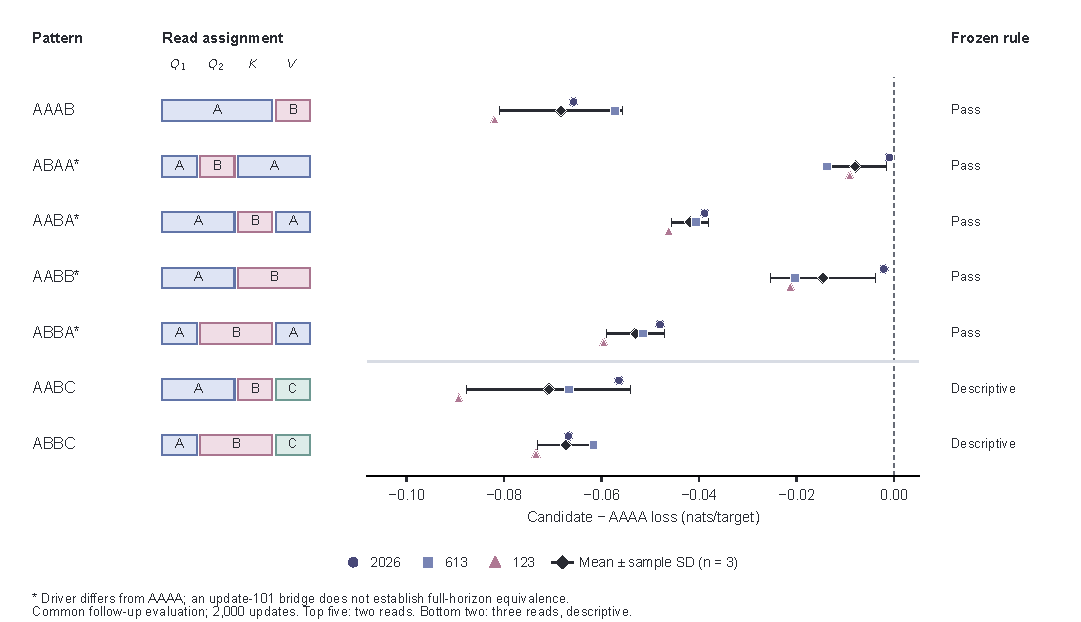
\includegraphics[width=\textwidth]{figures/all-read-effects.pdf}
\caption{Paired loss differences from shared-read MHAR at 2,000 updates.
Colored blocks show read assignments in $(Q_1,Q_2,K,V)$ order;
adjacent consumers sharing a read occupy one merged block.
Symbols show individual seeds; diamonds and whiskers show mean $\pm$ sample
SD, not confidence intervals. All five two-read patterns meet the frozen
practical rule; the three-read rows are descriptive. $^{*}$Cross-driver
comparison; the update-101 bridge does not establish endpoint equivalence.
Rows share the evaluation artifact and three \route{AAAA} references.}
\label{fig:all-effects}
\end{figure}

\subsection{Which consumers should share two reads?}
\label{sec:assignment}
All four new two-read patterns let $V$ share with another consumer and have
lower recorded loss than \route{AAAA} in every seed. Observed improvements
are therefore not confined to singleton-$V$ assignments; these parent contrasts
remain cross-driver. \route{AAAB} has the
lowest observed two-read mean. Its ranking against the four new patterns
remains cross-driver and descriptive; no pairwise criterion establishes an
optimal assignment.

Among the four additional two-read patterns, the ordering
$\route{ABBA}<\route{AABA}<\route{AABB}<\route{ABAA}$ holds in every
seed. These models share parameter count, read count, query-projection
layout and driver. Read count alone therefore does not explain their
quality differences. For the observed endpoints of this ordering,
\route{ABBA} minus \route{ABAA} is
$\WithinDriverMean\pm\WithinDriverSD$ nats/target (mean $\pm$ sample SD).
This contrast was selected after observing the results; it is descriptive,
not another promotion test. The patterns change several consumer couplings
together and do not isolate the effect of any one shared edge.
Figure~\ref{fig:fixed-read-effects} shows all four endpoint groups and their six paired contrasts.

\begin{figure}[!ht]
\centering
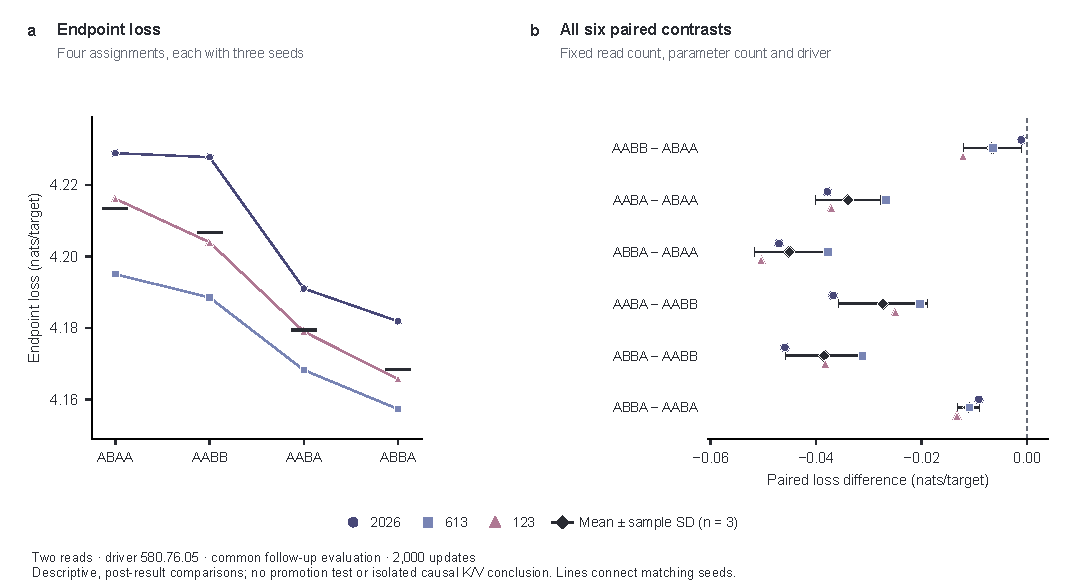
\includegraphics[width=\textwidth]{figures/fixed-read-effects.pdf}
\caption{Assignment at fixed read count and driver. (a) All twelve additional two-read
endpoints; lines connect the same training seed across categorical assignments,
not optimizer time. Short black marks denote condition means. (b) All six
paired contrasts among these four conditions. Symbols denote seeds; diamonds
and whiskers denote mean $\pm$ sample SD ($n=3$), not confidence intervals.
All conditions use two reads, the same parameter count, query-projection layout
and driver 580.76.05. These post-result comparisons are descriptive; they
add no promotion test and do not isolate a causal K/V effect.}
\label{fig:fixed-read-effects}
\end{figure}


\subsection{Does a finer allocation improve further?}
\label{sec:validation}
The three-read replication study tests \route{ABBC}, selected in the archival screen,
against \route{AAAB} and same-count \route{AABC} on the original primary.
Its \route{ABBC}--\route{AAAB} difference is
$\FreshPrimaryMean\pm\FreshPrimarySD$.
Seed 123 reverses the sign, and the mean misses the required $-0.0025$ margin.
The \route{ABBC}--\route{AABC} difference is
$+\FreshAllocationMean\pm\FreshAllocationSD$; its $-0.0015$ criterion also
fails. The original decisions remain failed.

On the common follow-up, the same checkpoints give mean differences
$+\FollowABBCvsAAAB{}$ and $+\FollowABBCvsAABC{}$, with the same per-seed sign patterns.
\route{AABC} has the lowest overall mean but beats \route{AAAB} in only
two seeds: its mean difference is $\FollowAABCvsAAAB{}$, with $+\AABCSeedReversal{}$ in seed
2026. Neither three-read pattern improves on \route{AAAB} in every seed.
The additional read therefore lacks a consistent incremental benefit in
this matrix. \route{AABC} remains descriptive, and the three patterns have
not been tested for equivalence.
Figure~\ref{fig:fresh-effects} separates the frozen tests from descriptive
follow-up contrasts. Original per-seed results remain in Appendix~\ref{app:scores}.

\begin{figure}[!ht]
\centering
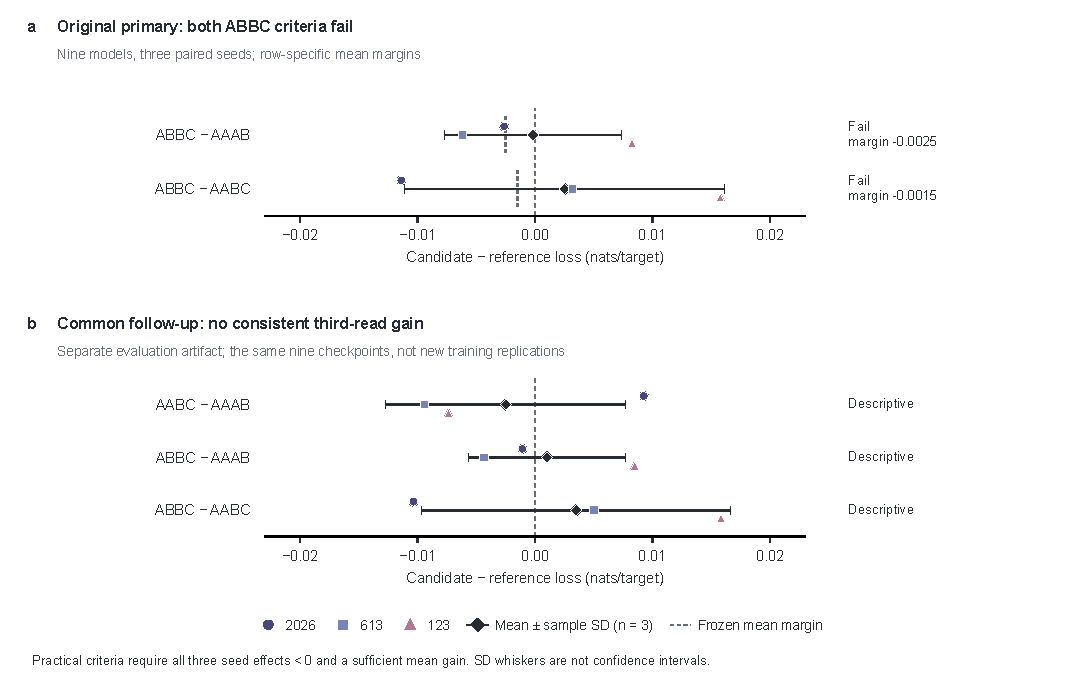
\includegraphics[width=\textwidth]{figures/fresh-seed-effects.pdf}
\caption{Incremental three-read comparisons at 2,000 updates. (a) The two
frozen original-primary contrasts both fail their criteria. Short dashed lines
mark the row-specific required mean differences; each rule also requires
negative differences in all three seeds. (b) Three descriptive contrasts on the
separate common follow-up artifact, including $\route{AABC}-\route{AAAB}$.
The same nine checkpoints are reused between panels; these are not independent
training replications, and artifact losses are not pooled. Symbols show seeds;
diamonds and whiskers show mean $\pm$ sample SD ($n=3$), not confidence
intervals. Negative favors the first-named model. Failure to establish
improvement is not an equivalence result.}
\label{fig:fresh-effects}
\end{figure}

\subsection{How do differences evolve during early training?}
\label{sec:dynamics}
Figure~\ref{fig:training-effects} follows paired batch training losses
through the observed 2,000 updates. For \route{AAAB}, \route{AABC} and
\route{ABBC}, mean gains over \route{AAAA} exceed 0.12 nats around updates
1,200--1,400, then narrow to about 0.071--0.073 nats in the final bin.
The other two-read patterns also show different trajectories. These are
training-loss curves, not repeated held-out evaluations or evidence of
convergence. The endpoint learning rate remains \LastLRPercent{}\% of peak;
the curves do not establish persistence or ranking over the full schedule.
Sampling and binning are specified in Appendix~\ref{app:training-curves}.

\begin{figure}[!ht]
\centering
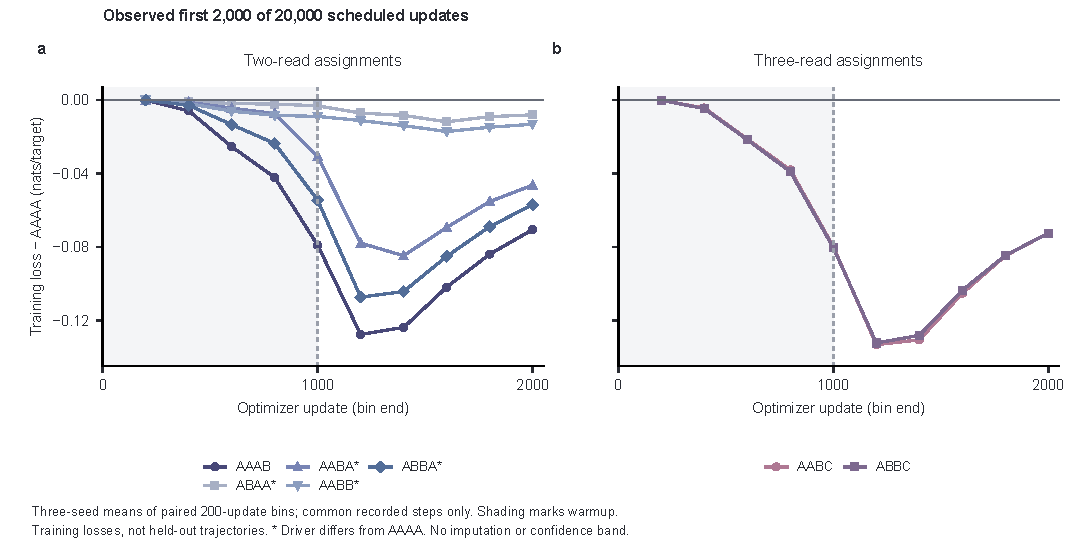
\includegraphics[width=\textwidth]{figures/training-read-effects.pdf}
\caption{Mean paired training-loss differences from \route{AAAA}, using
common recorded steps and 200-update bins (Appendix~\ref{app:training-curves}). Curves
average three seed differences; no confidence band is implied. Panels
separate two-read and three-read patterns. The vertical line and pale shading mark the 1,000-update warmup. $^{*}$Driver differs from the \route{AAAA} references.
These are batch training losses, not repeated primary evaluations.}
\label{fig:training-effects}
\end{figure}

\subsection{Does the value read use a distinct depth mixture?}
\label{sec:source-profiles}
Post-result forward probes expose the source weights of the six trained
\route{AAAB}/\route{ABBC} checkpoints on 32 fixed common-follow-up
sequences. The three-read \route{ABBC} comparison
(Figure~\ref{fig:source-depth-abbc}) distinguishes $A\to Q_1$,
$B\to Q_2,K$ and $C\to V$. All three reads have separate learned
pseudo-queries over the same source pool. Nevertheless, $A$ and $B$ are closer to
each other than either is to $C$: their mean half-L1 distances after token
averaging are \ProfileABBCHalfAB{}, \ProfileABBCHalfAC{} and
\ProfileABBCHalfBC{}, respectively. This ordering holds in each sampled seed.

The two-read \route{AAAB} comparison
(Figure~\ref{fig:source-depth-aaab}) shows the corresponding separation
between the shared $Q_1,Q_2,K$ read and the $V$ read, with mean half-L1
distance \ProfileAAABHalfLone{}. Across both assignments, the value-assigned
read gives more mass to the embedding and earlier MLP branches; the other
reads give more mass to earlier attention branches in the layer-averaged
sampled weights. This source-kind ordering also holds in each sampled seed.

Together, the profiles support a distinct source-access pattern for the
value-assigned read in these checkpoints. They do not isolate a causal effect
of assigning a read to $V$ or explain the loss differences. The maps average
tokens, sequences, feature heads and seeds; the reported distances further
average choice-bearing layers. Those cells are not independent training
replications. Probe definitions and passivity checks are in
Appendix~\ref{app:source-profiles}.

\begin{figure}[!htbp]
\centering
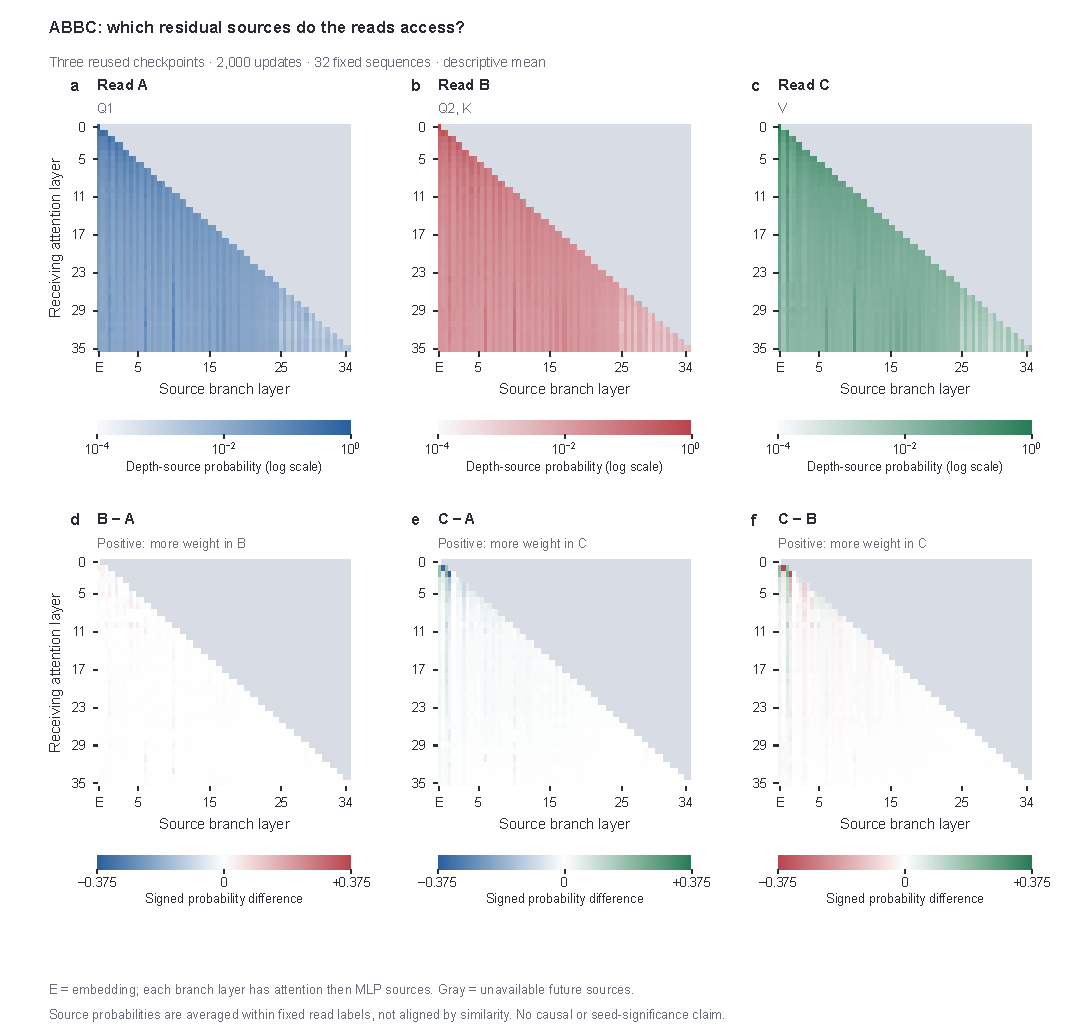
\includegraphics[width=\textwidth]{figures/source-depth-abbc.pdf}
\caption{Source-depth access in \route{ABBC}. (a--c) Blue $A$ feeds $Q_1$,
red $B$ feeds $Q_2,K$, and green $C$ feeds $V$. (d--f) Signed differences
$B-A$, $C-A$ and $C-B$; positive favors $B$, $C$ and $C$, respectively.
Rows are receiving attention layers; columns are the embedding ($E$), then
attention and MLP outputs of each earlier layer. Gray denotes unavailable
future sources. Probabilities share a logarithmic $[10^{-4},1]$ scale;
all signed maps use one symmetric linear scale. Cells equally average
1,023 query positions, 32 fixed sequences, eight MHAR feature heads and
three reused training seeds. Value-assigned $C$ is more distinct from the
other reads than they are from each other under the descriptive distance
in Equation~\ref{eq:profile-distance}. These access weights are not a causal
test or evidence of \route{ABBC} superiority.}
\label{fig:source-depth-abbc}
\end{figure}

\begin{figure}[!htbp]
\centering
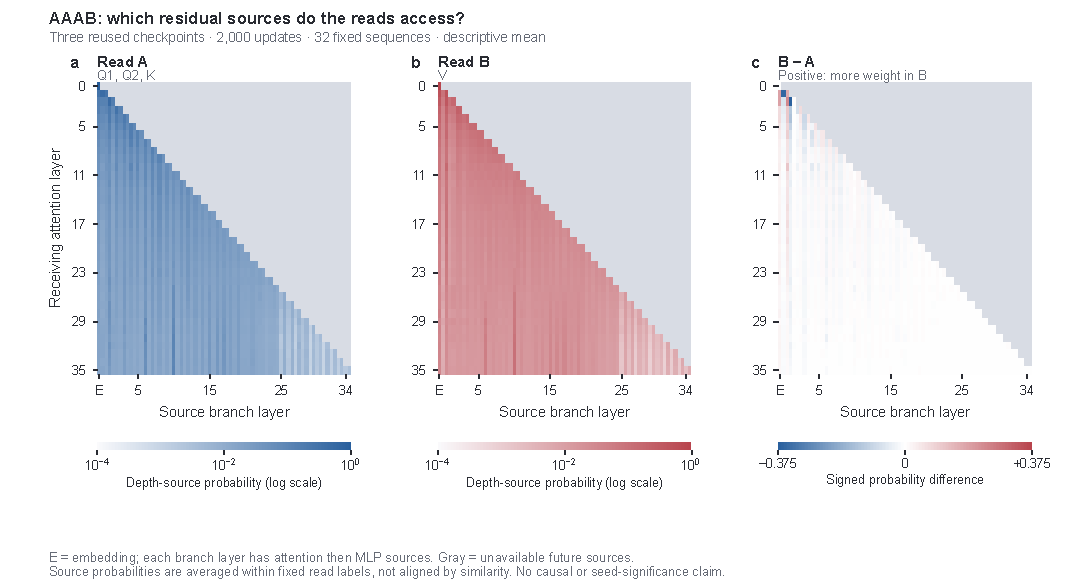
\includegraphics[width=\textwidth]{figures/source-depth-aaab.pdf}
\caption{Actual source-depth weights in \route{AAAB}. (a) Blue $A$ feeds
$Q_1,Q_2,K$; (b) red $B$ feeds $V$; (c) $B-A$, with positive values favoring
$B$. Axes, masks, probability limits, signed-difference limits and averaging
match Figure~\ref{fig:source-depth-abbc}. The value read is distinct from the
joint query/key read; \route{ABBC} additionally shows how the two addressing
reads compare with each other. These are mean source weights, not mean
tokenwise entropy. Head/seed averaging can hide heterogeneous differences.
Both figures reuse existing checkpoints and add no training or loss scores.}
\label{fig:source-depth-aaab}
\end{figure}
\paragraph{Archival tokenwise diagnostics.}
A complementary seed-42 probe of \route{ABBC}
(Figure~\ref{fig:route-abbc}) measures concentration and read differences
before averaging tokens. Value-assigned $C$ has lower mean normalized
entropy than $A$ or $B$, while the mean source-distribution JS divergence
between $A$ and $B$ is smaller than either pair involving $C$.
The archival confirmation view retains these mean orderings. This is a
single-checkpoint diagnostic, distinct from the three-seed source-weight
maps above; it does not explain their loss differences or establish
\route{ABBC} superiority. Appendix~\ref{app:route-profiles} defines these
averages and their relationship to the mean-weight maps.

\begin{figure}[!htbp]
\centering
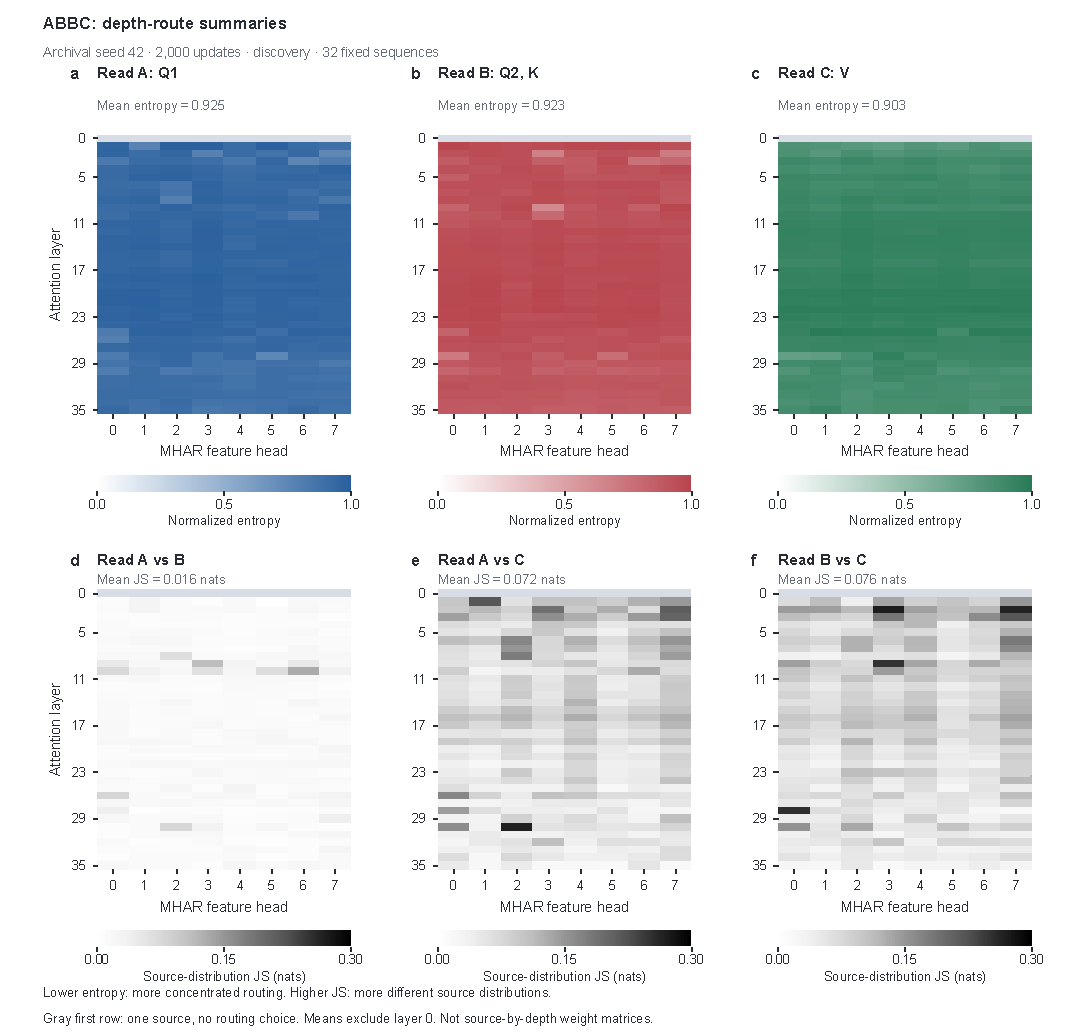
\includegraphics[width=\textwidth]{figures/route-profiles-abbc.pdf}
\caption{Archival \route{ABBC} read profiles. Blue $A$ feeds $Q_1$, red
$B$ feeds $Q_2,K$, and green $C$ feeds $V$. (a--c) Normalized individual-read
entropy on $[0,1]$; (d--f) all three pairwise source-distribution JS maps on
$[0,0.30]$ nats, without clipping. Cells average 1,023 valid query positions
per sequence, then 32 sequences. Layer 0 has only one source and is gray;
panel means equally weight layers 1--35 and eight feature heads. Darker colored cells
mean higher entropy; darker grayscale cells mean greater divergence.
$A$ and $B$ are closer on average than either is to $C$, with localized
differences across layers and feature heads. This is an archival
seed-42 single-checkpoint observation, not a replicated mechanism or evidence for
\route{ABBC} superiority. Colors identify reads, not positive or negative effects.}
\label{fig:route-abbc}
\end{figure}
\FloatBarrier

\section{Related Work}
\label{sec:related}
\paragraph{Depth readers and feature groups.}
AttnRes studies full and block-level source aggregation, including a
channel-group ablation~\cite{attnres2026}. % <!--ref:attnres2026--><!--anchor:section:3.2--><!--anchor:section:5.3-->
MHAR routes feature slices independently~\cite{mhar2026}. % <!--ref:mhar2026--><!--anchor:section:2.3-->
Its MHAR-HW variant gives each GQA group a full-width
read~\cite{mhar2026}. % <!--ref:mhar2026--><!--anchor:appendix:D-->
MSAR retrieves several full-width contextual streams and fuses them into
one sublayer input~\cite{msar2026}. % <!--ref:msar2026--><!--anchor:section:3.2-->
Depth Memory formalizes depth access through read/write operations and
implements an associative-memory readout added to the residual
input~\cite{depthmemory2026}. % <!--ref:depthmemory2026--><!--anchor:section:3.2-->
We retain the feature-sliced MHAR operator and assign its full-width outputs
to consumers within each GQA group, reusing the same reads across groups.

\paragraph{Role- and head-specific inputs.}
DeepCrossAttention supplies separate history aggregators for
$Q$, $K$ and $V$~\cite{dca2025}. % <!--ref:dca2025--><!--anchor:section:3.2-->
MUDDFormer generates dynamic connections for separate
$Q/K/V$/residual inputs~\cite{mudd2025}. % <!--ref:mudd2025--><!--anchor:section:2.2--><!--anchor:section:2.3-->
RD-AttnRes separates $QK$ and $V$ over Block-AttnRes
sources~\cite{rd2026}. % <!--ref:rd2026--><!--anchor:section:3-->
Our \route{AAAB} uses that sharing pattern under MHAR; it is not a matched
implementation of published RD-AttnRes.
DAGFormer gives individual query, key and value heads separate
coefficients over earlier layer outputs~\cite{dagformer2026}. % <!--ref:dagformer2026--><!--anchor:section:2.3-->
M3Former combines role-specific inputs with independent depth mixing for
feature groups assembled before projection; these groups are explicitly
distinct from attention heads~\cite{m3former2026}. % <!--ref:m3former2026--><!--anchor:section:2.2-->
These methods establish access at several granularities. Our comparison
fixes the reader and GQA organization, then varies which of
$(Q_1,Q_2,K,V)$ share its output.

\paragraph{Mixing attention projections and values.}
ExoFormer mixes reusable anchor and current $Q/K/V$/gate projections with
scalar, headwise or channelwise coefficients~\cite{exoformer2026}. % <!--ref:exoformer2026--><!--anchor:section:3.4-->
Depth-Attention mixes earlier-layer values inside attention using the
current query~\cite{depthattention2026}, % <!--ref:depthattention2026--><!--anchor:section:3.2-->
while Mixture-of-Depths Attention jointly attends to sequence and depth
KV entries~\cite{moda2026}. % <!--ref:moda2026--><!--anchor:section:2.2-->
Our assignments act on the hidden inputs to separate projections and retain
the native token-attention operation.

\paragraph{Residual states and recurrent depth.}
DAR retrieves from two histories using cross-stream scoring
keys~\cite{dar2026}. % <!--ref:dar2026--><!--anchor:section:3.2-->
Hyper-Connections mixes expanded parallel residual
states~\cite{hc2024}; % <!--ref:hc2024--><!--anchor:section:2.1--><!--anchor:section:2.2-->
mHC constrains that mixing with Sinkhorn
normalization~\cite{mhc2026}. % <!--ref:mhc2026--><!--anchor:section:4.2-->
HiRes separates residual width from compute width through block read/write
projections~\cite{hires2026}. % <!--ref:hires2026--><!--anchor:section:2.3-->
Multi-stream diffusion models study persistent residual streams and their
masked/visible-token roles~\cite{diffusionstreams2026}. % <!--ref:diffusionstreams2026--><!--anchor:section:3-->
InfiLoop aggregates recurrent candidates through content scores and temporal
decay~\cite{infiloop2026}; % <!--ref:infiloop2026--><!--anchor:section:3.1-->
StateLoop carries a persistent per-token state across
iterations~\cite{stateloop2026}. % <!--ref:stateloop2026--><!--anchor:section:3.1-->
Our attention reads draw on one source history without adding persistent
parallel residual streams.

\paragraph{KV grouping and reuse.}
AsymGQA uses activation-informed grouping when converting MHA to GQA,
changing which query heads share KV heads~\cite{asymgqa2024}. % <!--ref:asymgqa2024--><!--anchor:section:2.1-->
Cross-Layer Attention reuses KV activations across adjacent
layers~\cite{cla2024}. % <!--ref:cla2024--><!--anchor:section:2.2-->
WhiteMatter mixes layer histories into separately routed K/V channels
shared across layers~\cite{whitematter2026}. % <!--ref:whitematter2026--><!--anchor:section:3.1-->
AsymLoop combines fixed encoder global KV with iterative decoder local
KV~\cite{asymloop2026}. % <!--ref:asymloop2026--><!--anchor:section:3.1-->
We keep query-to-KV grouping and per-layer cache structure fixed.
External methods provide architectural context and are not measured
baselines in this study.

\paragraph{Causality of adaptive paths.}
Beyond Causal Masks identifies future-token leakage through sequence-wide
adaptive conditioning and studies prefix-invariance
audits~\cite{causalaudit2026}. % <!--ref:causalaudit2026--><!--anchor:section:7.5--><!--anchor:section:3-->
This validation property is separate from cache parity and checkpoint-resume
agreement.

\section{Discussion and Limitations}
\label{sec:discussion}
The completed matrix distinguishes untying reads from choosing their
assignment. All tested candidates improve on shared-read MHAR at the observed
endpoint, while equal-read comparisons show substantial differences between
assignments. \route{AAAB} is a useful two-read reference within this regime;
its best observed two-read mean does not establish a general optimum.
These effects are conditional on the $H=8$ MHAR parent and tested GQA ratio.
MHAR is not required to construct consumer-specific reads: RD-AttnRes
separates $QK$ and $V$ using Block AttnRes~\cite{rd2026}. % <!--ref:rd2026--><!--anchor:section:3-->
Our matrix does not compare matched single-head and multi-head depth readers.
It therefore does not establish whether feature-wise routing increases the
benefit of consumer separation or changes the ranking of sharing patterns.
A conventional additive-residual Transformer and matched implementations
of published alternatives are not measured baselines here.

One exploratory association merits a prospective test. Among the four
additional two-read patterns,
\route{AABA} and \route{ABBA} separate $K$ from $V$, whereas \route{ABAA}
and \route{AABB} tie them. Averaging each pair within each seed, then taking
separated minus tied and averaging over seeds, gives $\KVGroupedMean{}$
nats/target, favorable in all three seeds. The grouping was chosen after
observing the completed matrix. It changes query sharing as well as $K/V$
sharing and supplies no isolated causal effect or additional predeclared
test. Both $K/V$-tied alternatives still beat \route{AAAA}, so the pattern
concerns the size of the gain rather than a requirement for improvement.

Untying routing queries lets consumer groups adapt depth mixtures separately.
A shared query collects gradients from all its consumers; reducing a possible
compromise is a plausible explanation, not a measured mechanism here.
Optimization conditioning, router capacity and runtime differences remain
alternatives. Equal-read comparisons remove parameter-count differences among
the two-read patterns, but do not remove extra work/capacity versus \route{AAAA}.
The driver difference further limits cross-campaign attribution.

The horizon is the main limit on interpretation. Each model sees 65.5M input
positions, about 0.061 supervised targets per parameter, and half its updates
are in warmup. The last learning rate is \LastLRPercent{}\% of peak.
Training-loss gaps grow and then narrow within this window
(Section~\ref{sec:dynamics}). The endpoint losses establish early quality
differences; persistence through a completed schedule remains unmeasured.
Three fixed seeds, one corpus/model setting, reused checkpoints and evaluation
documents from one exclusion pool also limit generality. Document-ID
exclusion is not a near-duplicate audit, and seed 123 had prior engineering
exposure (Appendix~\ref{app:protocol}). Longer-horizon comparisons on one
driver, equal-compute evaluation and matched external methods remain open.

The archival full-width two-read and three-read screens motivated the fresh
comparisons rather than providing independent seed replication
(Appendix~\ref{sec:results}). Earlier feature-access controls and
separate-reader interventions distinguish three questions: which features
a projection can read, which consumers share a read, and whether a trained
checkpoint depends on that read (Appendix~\ref{app:historical-controls}).
Dependence alone is insufficient: request-conditioned and contrast-readout
controls use their added mechanisms without a confirmed gain over their parent. The
cache-matched feature-local attention extension also worsens loss and timing
(Appendix~\ref{app:compound}); its simultaneous graph changes do not isolate
feature locality. These development results are not pooled with the 24-model
comparison.

\section{Conclusion}
\label{sec:conclusion}
The tested depth-read assignments show unequal early-training gains under fixed
GQA and MHAR. All five tested two-read assignments have lower loss than the
shared-read parent at 2,000 updates, including four where $V$ shares its read.
Those four comparisons with the parent remain cross-driver; their mutual
ordering is consistent across seeds on one driver. Neither tested three-read
pattern establishes a consistent incremental gain over \route{AAAB}, and the
$K/V$-sharing association remains exploratory. The evidence favors studying the
sharing assignment alongside read count, with longer-horizon and equal-compute
outcomes open.

\section*{Availability and Disclosures}
Appendix~\ref{app:scores} reports all 33 endpoint scores from the 24 trained models.
The code, configurations and per-seed results are in the repository linked on
the title page. The repository is currently private and is planned for public
release. Release terms for data and checkpoints remain to be finalized.
AI assistance was used for analysis, drafting, source checks, manuscript
review and LaTeX preparation.

\clearpage
\appendix
\section{Full Model Definition}
\label{app:model}
This appendix specifies the MHAR operator, normalization and physical head
layout used in Equation~\ref{eq:sharing-inputs}.

\subsection{A depth read and its feature-routing heads}
We suppress the batch index and use zero-based layer indices
$\ell=0,\ldots,L-1$ and token positions $t=0,\ldots,T-1$. The model width is
$D=1,280$ over $L=36$ layers. There are $H=8$ MHAR feature-routing heads,
and each contiguous feature slice has width $d_r=D/H=160$.
These are different quantities from the
$G=8$ GQA groups and the $d_a=80$ token-attention head width, with two query
heads per group and $2Gd_a=D$.
Except where native weights or casts are specified, the equations describe
the real-arithmetic graph; they do not replace the recorded finite-precision
execution policy. Feature and token-head coordinates are zero-based.

Let $x_t\in\{0,\ldots,\mathcal V-1\}$ be a token ID, where
$\mathcal V=151{,}936$, and let $E\in\mathbb R^{\mathcal V\times D}$ be the
embedding matrix, so $e_t=E_{x_t,:}^{\mathsf T}\in\mathbb R^D$.
Let $a_{j,t},m_{j,t}\in\mathbb{R}^{D}$ be the retained \emph{branch outputs} of
attention and MLP in layer $j$. For the full-history MHAR model,
the ordered source lists, each containing $D$-vectors at position $t$, are
\begin{align}
 \mathcal{S}^{\mathrm{attn}}_{\ell,t}
   &= (e_t,a_{0,t},m_{0,t},\ldots,a_{\ell-1,t},m_{\ell-1,t}),\\
 \mathcal{S}^{\mathrm{mlp}}_{\ell,t}
   &= \mathcal{S}^{\mathrm{attn}}_{\ell,t}\mathbin{\Vert}(a_{\ell,t}).
 \label{eq:sources}
\end{align}
Here $\Vert$ denotes list concatenation and
$\mathcal{S}^{\mathrm{attn}}_{0,t}=(e_t)$, with source counts
$N^{\mathrm{attn}}_\ell=2\ell+1$ and $N^{\mathrm{mlp}}_\ell=2\ell+2$.
These lists contain embedding/branch-output candidates, not cumulative
residual sums or a separate history per read. The MLP keeps its native single read. All compared all-global
graphs use this same source construction.

For a vector $x\in\mathbb{R}^{n}$ and learned scale
$\gamma\in\mathbb{R}^{n}$, write the mathematical RMS normalization as
\begin{equation}
 \mathcal{N}_{\gamma}(x)
 =\gamma\odot\frac{x}{\sqrt{\epsilon+n^{-1}\sum_{k=0}^{n-1}x_k^2}},
 \qquad \epsilon=10^{-6}.
 \label{eq:rmsnorm}
\end{equation}
There is no additive normalization bias. Distinct source, branch-input and
head-normalization modules have their own scale vectors. The RMS statistic
is accumulated in FP32 and the normalized tensor is cast
back before scale multiplication; Equation~\ref{eq:rmsnorm} describes the
operation, not all finite-precision rounding boundaries.

At an attention site, let $s_{\ell i t}$ be source $i$ from
$\mathcal{S}^{\mathrm{attn}}_{\ell,t}$, with $i=0,\ldots,N^{\mathrm{attn}}_\ell-1$.
For slice $I_h=\{(h-1)d_r,\ldots,hd_r-1\}$, $h=1,\ldots,H$, and read
$r\in\{A,\ldots\}$, the learned pseudo-query is
$q^r_{\ell h}\in\mathbb{R}^{d_r}$. The read is
\begin{align}
 \kappa_{\ell i t}
   &=\mathcal{N}_{\gamma^{\mathrm{depth,attn}}_\ell}(s_{\ell i t}),\\
 \eta^r_{\ell iht}
   &=\left\langle q^r_{\ell h},[\kappa_{\ell i t}]_{I_h}\right\rangle,\\
 \alpha^r_{\ell iht}
   &=\frac{\exp(\eta^r_{\ell iht})}
   {\sum_{v=0}^{N^{\mathrm{attn}}_\ell-1}\exp(\eta^r_{\ell vht})},\\
 h^r_{\ell,t}
   &=\operatorname{concat}_{h=1}^{H}
   \left(\sum_{i=0}^{N^{\mathrm{attn}}_\ell-1}
   \alpha^r_{\ell iht}[s_{\ell i t}]_{I_h}\right)
   \in\mathbb{R}^{D}.
 \label{eq:read}
\end{align}
The source RMS statistic is computed over the full width $D$ \emph{before}
slicing, not independently within each $d_r$-slice. It is shared across reads
at the site. Softmax is over residual sources only, separately for every
$(r,h,t)$; the score has no $d_r^{-1/2}$ factor, source-dependent logit bias or
token-query projection. Values are the raw source slices, not normalized keys.
Each read has $D$ pseudo-query parameters and remains full-width after
concatenation. Write $q^r_\ell\in\mathbb R^{H\times d_r}$ for the
collection of its $H$ pseudo-query vectors. We denote this same operator on any ordered source list by
$\mathcal{D}(\mathcal{S};q,\gamma)$, with $H$ fixed and the indicated query and
source-normalization parameters. Equations~\ref{eq:sources}--\ref{eq:read}
use the full branch-output history rather than Block-AttnRes sources.

\subsection{Consumer sharing under fixed GQA}
Let $\mathcal{C}=\{Q_1,Q_2,K,V\}$ be the consumers of one group and
$\mathcal{R}$ the set of $R$ read identities. A surjective assignment
$\rho:\mathcal{C}\to\mathcal{R}$ induces the sharing partition
\begin{equation}
 c\sim_\rho c'\quad\Longleftrightarrow\quad\rho(c)=\rho(c').
 \label{eq:sharing}
\end{equation}
Sharing means using the same parameterized read, not merely obtaining equal
values on a particular input. Independently parameterized reads can produce
identical mixtures at initialization or on individual tokens without being
the same read.

At each attention site, the model constructs $R$ full-width states
$\{h^r_{\ell,t}:r\in\mathcal{R}\}$ in total and reuses them across all eight
GQA groups. It does \emph{not} construct $R$ independent reads per group.
Group-specific projection rows consume the branch-normalized states:
\begin{align}
 x^r_{\ell,t}
   &=\mathcal{N}_{\gamma^{\mathrm{in,attn}}_\ell}(h^r_{\ell,t}),\\
 \widetilde Q_{\ell,g,j,t}
   &=W^Q_{\ell,g,j}x^{\rho(Q_j)}_{\ell,t},\quad j\in\{1,2\},\\
 \widetilde K_{\ell,g,t}
   &=W^K_{\ell,g}x^{\rho(K)}_{\ell,t},
 &V_{\ell,g,t}&=W^V_{\ell,g}x^{\rho(V)}_{\ell,t}.
 \label{eq:consumers}
\end{align}
Here $g=0,\ldots,G-1$ and each $W^Q_{\ell,g,j},W^K_{\ell,g},W^V_{\ell,g}$
has shape $d_a\times D$. The input RMSNorm scale is shared between reads, but
is separate from the depth-source scale in Equation~\ref{eq:read}. No residual
interpolation or depth-logit bias is applied. All $Q/K/V/O$ projection biases
are disabled in these comparisons.

The token-attention queries and keys then receive learned head-width RMSNorm
and RoPE, in that order:
\begin{align}
 \widehat Q_{\ell,g,j,t}
   &=\operatorname{RoPE}_t\!\left(
     \mathcal{N}_{\gamma^Q_\ell}(\widetilde Q_{\ell,g,j,t})\right),\\
 \widehat K_{\ell,g,t}
   &=\operatorname{RoPE}_t\!\left(
     \mathcal{N}_{\gamma^K_\ell}(\widetilde K_{\ell,g,t})\right).
 \label{eq:qk-norm-rope}
\end{align}
The two scale vectors $\gamma^Q_\ell,\gamma^K_\ell\in\mathbb{R}^{d_a}$ are
distinct: the first is shared across all 16 query heads, the second across
all eight key heads. There is no corresponding head RMSNorm or RoPE on $V$.
The native RoPE uses split-half coordinate pairs, rather than adjacent
coordinate pairs. For $v\in\mathbb R^{d_a}$ and $k=0,\ldots,d_a/2-1$,
its ideal-arithmetic definition is
\begin{align}
 \omega_k&=10{,}000^{-2k/d_a}, &\varphi_{t,k}&=t\omega_k,\\
 [\operatorname{RoPE}_t(v)]_k
   &=v_k\cos\varphi_{t,k}-v_{k+d_a/2}\sin\varphi_{t,k},\\
 [\operatorname{RoPE}_t(v)]_{k+d_a/2}
   &=v_{k+d_a/2}\cos\varphi_{t,k}+v_k\sin\varphi_{t,k}.
 \label{eq:rope}
\end{align}
There is no frequency scaling. Cosine/sine buffers retain their native
precision and cast boundaries across checkpoint reloads.
For an unpadded causal prefix,
\begin{align}
 \beta_{\ell,g,j,t,u}
   &=\frac{\exp\!\left(
      \widehat Q_{\ell,g,j,t}^{\mathsf T}\widehat K_{\ell,g,u}/\sqrt{d_a}\right)}
     {\sum_{v=0}^{t}\exp\!\left(
      \widehat Q_{\ell,g,j,t}^{\mathsf T}\widehat K_{\ell,g,v}/\sqrt{d_a}\right)},
      \quad 0\leq u\leq t,\\
 o_{\ell,g,j,t}&=\sum_{u=0}^{t}\beta_{\ell,g,j,t,u}V_{\ell,g,u},\\
 a_{\ell,t}&=W^O_\ell\operatorname{concat}_{g=0}^{G-1}
       (o_{\ell,g,2,t},o_{\ell,g,1,t}).
 \label{eq:token-attention}
\end{align}
The $d_a^{-1/2}$ scaling belongs to token attention, not depth routing.
Attention dropout is zero. Both query consumers use the same $K_g,V_g$, while
each produces its own token-attention map. The even/odd order in the
concatenation follows the implementation's physical query-head layout.
During cached inference, each group stores only the normalized/rotated
$\widehat K_{\ell,g,u}$ and the projected $V_{\ell,g,u}$, without one cache
stream per depth read. These equations state the all-global graph; backend
casting and reduction order remain part of its separate numerical binding.

Letters label the $R$ read identities, without intrinsic meaning.
For example, \route{ABBC} means $\rho(Q_1)=A$, $\rho(Q_2)=\rho(K)=B$, and $\rho(V)=C$.
The template is fixed across layers and groups; it is not a learned per-group
topology. Logical $Q_1$ maps to physical head $2g+1$ and $Q_2$ to $2g$ in both
the archival and fresh implementations.
The asymmetry is between one query and the other, not a claim that a particular
query-head label has an intrinsic semantic role.

Route relabeling and exchange of query slots reduce the up-to-two-read space to
one shared-read parent and five two-read classes, all shown in
Table~\ref{tab:two}. There are seven unlabeled nonempty bipartitions of four
consumers; exchanging the query slots identifies two pairs, leaving five
classes. Query exchange is an
architecture symmetry only with the corresponding query-projection rows and
output-projection columns exchanged. It does not imply that two unpermuted
initializations have identical training trajectories. The archival equivalence
fixtures justify the class coverage, not seed robustness.

\subsection{History updates, the MLP, and the final readout}
The attention output $a_{\ell,t}$ in Equation~\ref{eq:token-attention} is
appended as one new source. The MLP uses one unchanged MHAR read with its own
pseudo-query and source RMSNorm, followed by its own input RMSNorm and native
gated feed-forward branch:
\begin{align}
 b_{\ell,t}
   &=\mathcal{D}(\mathcal{S}^{\mathrm{mlp}}_{\ell,t};
        q^{\mathrm{mlp}}_\ell,\gamma^{\mathrm{depth,mlp}}_\ell),\\
 y_{\ell,t}&=\mathcal{N}_{\gamma^{\mathrm{in,mlp}}_\ell}(b_{\ell,t}),\\
 m_{\ell,t}&=W^{\mathrm{down}}_\ell
       \left[\phi(W^{\mathrm{gate}}_\ell y_{\ell,t})
       \odot(W^{\mathrm{up}}_\ell y_{\ell,t})\right],\\
 \mathcal{S}^{\mathrm{attn}}_{\ell+1,t}
   &=\mathcal{S}^{\mathrm{mlp}}_{\ell,t}\mathbin{\Vert}(m_{\ell,t}).
 \label{eq:branch-updates}
\end{align}
Here $W^{\mathrm{gate}}_\ell,W^{\mathrm{up}}_\ell$ have shape
$5,120\times D$, $W^{\mathrm{down}}_\ell$ has shape $D\times5,120$, and
$\phi(z)=z\,\sigma(z)$ is SiLU, with $\sigma(z)=(1+e^{-z})^{-1}$ applied
elementwise. All three MLP projections are bias-free. Branch outputs enter
the shared depth-source history once, without being added to their input reads.
This is why Equation~\ref{eq:sources} is a branch-output list rather than a
conventional sequence of cumulative residual sums.

After all $L=36$ layers, the native backbone performs one final MHAR read over
the embedding and all $2L$ branch outputs, then output RMSNorm and the LM head:
\begin{align}
 f_t&=\mathcal{D}(\mathcal{S}^{\mathrm{attn}}_{L,t};
           q^{\mathrm{out}},\gamma^{\mathrm{depth,out}}),
 &|\mathcal{S}^{\mathrm{attn}}_{L,t}|&=2L+1=73,\\
 z_t&=W^{\mathrm{LM}}\mathcal{N}_{\gamma^{\mathrm{out}}}(f_t),
 &p_\theta(\cdot\mid x_{\leq t})&=\operatorname{softmax}(z_t).
 \label{eq:final-readout}
\end{align}
The final read uses the same feature-sliced operator but its own query and
source-normalization parameters. It is common to all compared topologies and
does not create an additional consumer-specific output head. The LM head is
tied to the embedding matrix, $W^{\mathrm{LM}}=E$.
Changes in attention read assignment can
change subsequent branch outputs and therefore their histories; sharing the
history construction does not assert equal historical tensors between models.

\subsection{Coverage of the partition space}
Under the same symmetries, there are four three-read classes and one four-read
class, giving $1+5+4+1=11$ in total (Figure~\ref{fig:topology}). The three-read
screen tests \route{AABC} and \route{ABBC}; it does not test
\route{ABCA}, $(Q_1V)\mid Q_2\mid K$, or
\route{ABCC}, $Q_1\mid Q_2\mid(KV)$. The four-read
\route{ABCD}, $Q_1\mid Q_2\mid K\mid V$, is also untested. Coverage of all
two-read classes therefore does not imply an exhaustive topology search or a
globally optimal selected graph.

\begin{figure}[!ht]
\centering
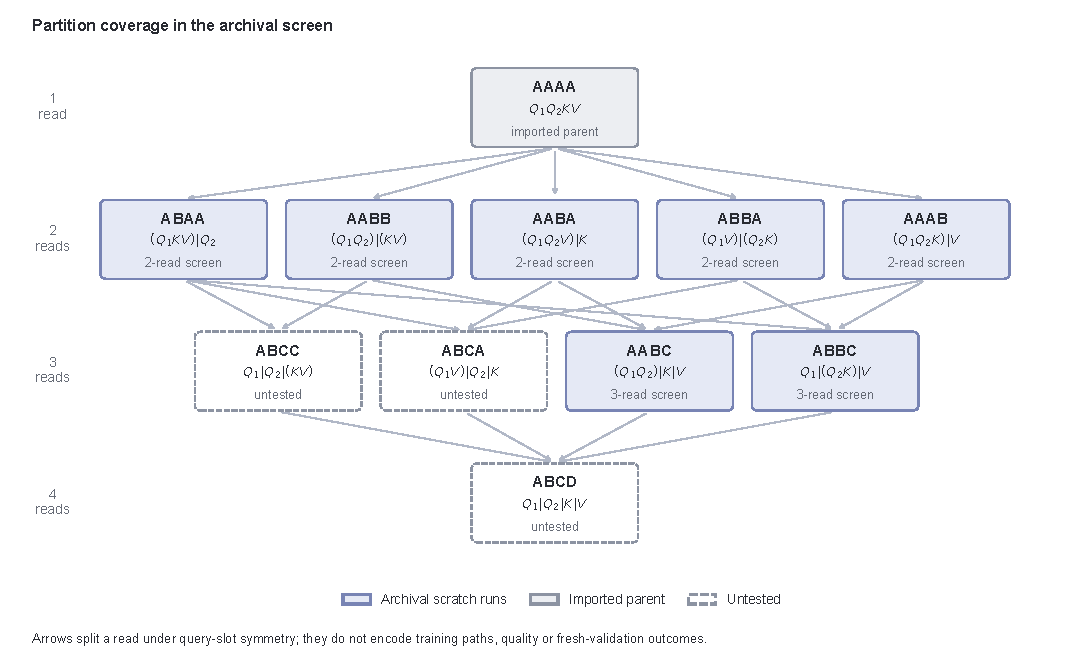
\includegraphics[width=\textwidth]{figures/topology-space.pdf}
\caption{Archival coverage of the complete consumer-sharing space modulo route-label permutation and
exchange of the two query slots. Filled pale nodes have archival scratch-run
evidence; gray \route{AAAA} is an imported historical parent; white dashed
nodes are untested in the reported screen. Arrows indicate that some
representative of the target class splits one read of a representative of the
source class. They do not encode a training trajectory, quality ranking, or
fresh-validation outcome. In particular, gray \route{AAAA} was imported in the
archival screen; its three newly trained controls belong to the later shared-read follow-up,
not this historical coverage map. Query exchange requires the corresponding $Q$ rows
and output-projection columns to be permuted; graph equivalence alone does not
imply identical independently seeded optimization trajectories.}
\label{fig:topology}
\end{figure}

\subsection{What an extra read costs}
Each added attention read contributes $D$ query parameters and one score and
one value-mixture dot product per source and token. Across $L$ layers,
\begin{align}
 \Delta P&=LD=46{,}080,\\
 \Delta\mathrm{MAC}_{\mathrm{forward/token}}
   &=2D\sum_{\ell=0}^{L-1}(2\ell+1)
     =2DL^2=3{,}317{,}760,\\
 \Delta M_{\mathrm{state/site}}&=BTD\,b_{\mathrm{elem}}.
 \label{eq:read-cost}
\end{align}
Here $B$ is batch size and $b_{\mathrm{elem}}=2$ bytes for BF16.
Both one-to-two and two-to-three comparisons incur these per-read increments.
Backward and checkpoint-replay work is additional. A MAC denotes one multiply-accumulate;
counting its multiply and add separately gives two FLOPs per MAC. This
score/mix count excludes normalization, softmax, data movement and launch costs.
One additional BF16 full-width state
at batch 4, length 1,024 occupies 10 MiB per site before autograd and other
workspace. These are analytical quantities, not measured latency or total VRAM.
The all-global packed KV payload at cached length $T_c$ is
\begin{equation}
 M_{\mathrm{KV}}=2BLG T_c d_a\,b_{\mathrm{elem}},
 \label{eq:kv-payload}
\end{equation}
with no factor $R$. This excludes residual-source history, allocator/workspace
overheads and other live tensors; it is not a total inference-memory estimate.
The archival backend executes three real reads using two two-read tiles,
including a dummy forward role. This is a possible implementation overhead,
not a profile-based attribution of the observed time difference. The fresh
canonical backend is a separate execution policy and does not inherit a
measured overhead ratio from that path.

In the archival implementation, tied query inputs use one full-output projection
GEMM; split inputs use two half-output GEMMs. The ideal projection work and
packed KV payload are unchanged, but the execution shapes differ. Thus even
the archival same-count comparison does not match query-GEMM layout.
\route{ABBC} versus \route{AAAB} changes both
read count and allocation; \route{ABBC} versus \route{AABC} holds read count
fixed. Neither comparison should be described as an isolated proof about one
consumer's causal role without the corresponding controls.

\section{Training and Evaluation Protocol}
\label{app:protocol}
\subsection{Training and supervision}
The learning-rate peak/minimum are $5\times10^{-4}/5\times10^{-5}$.
AdamW uses $(\beta_1,\beta_2)=(0.9,0.95)$, $\epsilon=10^{-8}$, weight decay
0.1 and global gradient $L_2$-norm clipping at 1.0 after accumulation.
Parameters and native AdamW moment tensors use BF16; there is no FP32
master-parameter copy or GradScaler. Gradient checkpointing is enabled;
compilation and FSDP are disabled. The tokenizer's model name does not
specify the trained model size (Table~\ref{tab:parameters}).

Let $k$ denote the number of completed updates. The learning rate used by
update $k+1$ is
\begin{equation}
 \eta(k)=5\times10^{-4}
 \begin{cases}
 k/1000,&0\leq k<1000,\\
 0.1+0.9\,\dfrac{1+\cos\!\left(\pi\dfrac{k-1000}{20000-1000}\right)}{2},
   &1000\leq k\leq20000.
 \end{cases}
 \label{eq:lr-schedule}
\end{equation}
The optimizer step precedes the scheduler step: update 1 uses $\eta(0)=0$,
and update 2,000 uses $\eta(1999)$, the recorded last-used rate. The scheduler
state after that update contains $\eta(2000)$; both are \LastLRPercent{}\%
of peak at the displayed precision.

Loss is token-weighted negative log-likelihood in nats/token. For input sequence
$x_{i,0},\ldots,x_{i,T-1}$ and model logits $z_{i,t}$ from
Equation~\ref{eq:final-readout}, the preserved supervision is
\begin{align}
 u_i(\theta)&=-\sum_{t=0}^{T-2}
       \log\!\left[\operatorname{softmax}(z_{i,t})\right]_{x_{i,t+1}},
 &n_i&=T-1=1{,}023,\\
 \Loss(\theta)&=\frac{\sum_i u_i(\theta)}{\sum_i n_i}.
 \label{eq:supervised-loss}
\end{align}
The last logit at position $T-1$ is ignored; the stored lookahead at raw
position $T$ is not a supervised target. Evaluation computes token cross-entropy
from FP32 logits and accumulates per-sequence totals in FP64. This convention
does not mask EOS or document-boundary transitions. Signed differences
are candidate minus named reference; negative is better.

\subsection{Matched initialization and execution}
The fixed three-read replication matrix is
\begin{equation}
 \{\route{AAAB},\route{AABC},\route{ABBC}\}
 \times\{2026,613,123\},
 \qquad 2{,}000\text{ updates per run}.
 \label{eq:fresh-matrix}
\end{equation}
The common parameters, query-slot rows and training-stream bytes are
matched within each seed. The initializer constructs the native model and
copies its attention routing query into additional reads without consuming
RNG. With the notation of Appendix~\ref{app:model},
\begin{equation}
 \begin{aligned}
 q_{\ell}^{A,\route{AAAB}}(0)=q_{\ell}^{B,\route{AAAB}}(0)
   &=q_\ell^{\mathrm{native}}(0),\\
 q_{\ell}^{r,\route{AABC}}(0)=q_{\ell}^{r,\route{ABBC}}(0)
   &=q_\ell^{\mathrm{native}}(0),\quad r\in\{A,B,C\}.
 \end{aligned}
 \label{eq:init-mapping}
\end{equation}
In real arithmetic, the native zero-query initialization gives
\begin{equation}
 q^r_{\ell h}(0)=0\quad\Longrightarrow\quad
 \alpha^r_{\ell iht}(0)=\frac{1}{N^{\mathrm{attn}}_\ell},\qquad
 h^r_{\ell,t}(0)=\frac{1}{N^{\mathrm{attn}}_\ell}
       \sum_i s_{\ell i t}(0).
 \label{eq:uniform-init}
\end{equation}
In native BF16, softmax stores the rounded value of $1/N^{\mathrm{attn}}_\ell$;
the subsequent mixture also follows native rounding. Thus the equation is
an ideal uniform-average identity, not a claim of exact unit probability
mass or bit equality with a separately evaluated arithmetic mean.
The copies are independently trainable. Query heads themselves are not
tied. All conditions use the same two 640-output query GEMMs, including
shared-input cases; logical $Q_2$ occupies even physical heads and $Q_1$ odd
heads. Training uses PyTorch 2.8.0+cu128, Transformers 4.57.6 and strict
determinism on an RTX 5090.
The additional two-read models use the same native-query copying rule;
common initial parameters, query-slot rows and training streams are matched
within each seed. The shared-read control has only its single active router.
Short-run continuation checks compare uninterrupted execution and two
independent resumes at update 101. These checks and strict determinism do
not establish full-horizon equivalence between drivers.

The seed list was amended from $123,2025,3407$ to $2026,613,123$ before
scientific training. Seed 123 had already been used for 100-update
engineering trials and continuations to update 101; their training metrics
were recorded before the amendment was first documented. All scientific
model and optimizer states start from scratch, with the seed-123 training
stream reused. Decision timing relative to prior metric access is not
independently established.

\subsection{Source pool and deterministic document selection}
\label{app:data-selection}
The ordered source shards are \path{sample/10BT/000_00000.parquet} and
\path{sample/10BT/001_00000.parquet} from FineWeb-Edu sample-10BT, revision
\texttt{87f09149}. The Qwen3-0.6B tokenizer revision is \texttt{c1899de2}.
Full revision IDs and artifact identities are provided in the companion
reproducibility materials. The sample-10BT configuration name does not mean
that every source shard or ten billion tokens was used.

The function \texttt{hash\_json} below returns the hexadecimal SHA-256 digest
of UTF-8 canonical JSON with sorted keys, compact separators and no ASCII
escaping. The namespace binds the dataset repository,
revision and configuration. For each nonempty source document, the identity
and selection rank are
\begin{quote}\small
\begin{verbatim}
uid  = hash_json(["native_id_v1", namespace, native_id])
rank = hash_json(["primary-selection-v1", selection_salt, uid])
excluded = first_4096_unique_ids(sorted_by=(rank, uid))
\end{verbatim}
\end{quote}
Conflicting text under one native identity is rejected. The selection salt is
\path{paper-sharing-fresh-2k-v1:primary:2026-10-14}. Selected documents are packed
in rank/identity order for the primary artifact. All occurrences of the
4,096 selected IDs are excluded before training shuffle and tokenization.
Each training stream uses its scientific seed with a 10,000-document buffer
under Datasets 4.5.0, then packs 64,000 windows. This is document-ID exclusion,
not semantic or near-duplicate decontamination.

\subsection{Evaluation freezes and checkpoint reuse}
The original primary artifact was frozen before the nine scratch trainings.
Source-document IDs are excluded before token packing; document identities,
ordering, tokenizer revisions, tokens and masks are hash-bound.
Every endpoint score contains 1,047,552 supervised targets.
All nine final checkpoints were bound before scoring. There was no
partial-matrix primary look, replacement candidate or rescue seed.

The follow-up artifact was frozen after the three-read replication outcome and
before follow-up scoring. Its pool contains the 3,090 unused members of the
original 4,096-document exclusion set, removing all 1,006 contributors to
the original primary. It contains 1,024 sequences from 973 contributing
documents. Recorded training-ID intersections are empty. The shared-read
study scores twelve subjects once on this artifact; the two-read assignment
study scores twelve additional
models on the same artifact and copies six existing reference scores
byte-for-byte. The nine original candidates retain their original-primary
scores and checkpoint identities. A second evaluation of those models is
not independent retraining or an independent corpus.

\subsection{Predeclared comparisons}
Let $\mathcal U=\{2026,613,123\}$. On the original primary artifact, the
three-read replication differences are
\begin{align}
 d_s &= \Loss_{\route{ABBC},s}-\Loss_{\route{AAAB},s}, &
 a_s &= \Loss_{\route{ABBC},s}-\Loss_{\route{AABC},s},\\
 \bar d &= \tfrac{1}{3}\sum_{s\in\mathcal U} d_s, &
 \bar a &= \tfrac{1}{3}\sum_{s\in\mathcal U} a_s.
 \label{eq:seed-contrasts}
\end{align}
Primary promotion requires
\begin{equation}
 \boxed{\forall s\in\mathcal U:\ d_s<0\quad\text{and}\quad\bar d\leq-0.0025.}
 \label{eq:primary-gate}
\end{equation}
The stronger allocation claim additionally requires
\begin{equation}
 \boxed{\forall s\in\mathcal U:\ a_s<0\quad\text{and}\quad\bar a\leq-0.0015.}
 \label{eq:allocation-gate}
\end{equation}
The paired sample SDs are
\begin{equation}
 s_d=\sqrt{\frac{\sum_{s\in\mathcal U}(d_s-\bar d)^2}{3-1}},
 \qquad
 s_a=\sqrt{\frac{\sum_{s\in\mathcal U}(a_s-\bar a)^2}{3-1}}.
 \label{eq:seed-sd}
\end{equation}
For the shared-read follow-up,
\begin{equation}
 b_s^c=\Loss^{\mathrm{followup}}_{c,s}
       -\Loss^{\mathrm{followup}}_{\route{AAAA},s},\qquad
 \bar b^c=\tfrac13\sum_{s\in\mathcal U}b_s^c.
 \label{eq:stage-a-contrast}
\end{equation}
The primary \route{AAAB} contrast requires every
$b_s^{\route{AAAB}}<0$ and $\bar b^{\route{AAAB}}\leq-0.0025$.
After the shared-read baseline study passes, the two-read assignment study
completes the frozen family
\begin{equation}
 \begin{gathered}
 \mathcal F_2=\{\route{AAAB},\route{ABAA},\route{AABA},\route{AABB},\route{ABBA}\},\\
 \bigwedge_{c\in\mathcal F_2}
 \left[(\forall s\in\mathcal U:\ b_s^c<0)\ \land\ (\bar b^c\leq-0.0025)\right].
 \end{gathered}
 \label{eq:two-read-family}
\end{equation}
The margin constrains each condition's \emph{mean}, not each seed's magnitude.
The \route{AABC}/\route{ABBC} rows remain descriptive. For an equally
seed-weighted loss contrast, $\mathrm{PPL}=\exp(\Loss)$ and the
geometric-mean perplexity reduction on the common follow-up artifact is
\begin{equation}
 100\left(1-\frac{\exp(\frac13\sum_{s\in\mathcal U}\Loss^{\mathrm{followup}}_{c,s})}
                       {\exp(\frac13\sum_{s\in\mathcal U}\Loss^{\mathrm{followup}}_{\route{AAAA},s})}\right)
 =100(1-\exp(\bar b^c)).
 \label{eq:geometric-ppl}
\end{equation}
This is the reduction in the geometric mean of paired perplexity ratios,
not the arithmetic mean of per-seed percentage reductions.
These practical criteria are not significance or equivalence tests.
No decision uses rounded values, sequence-bootstrap uncertainty in place of
seed variability, or a post-result threshold change.
With three paired seeds, even three favorable signs give a one-sided sign
probability of $1/8$ under independent fair signs. This illustrates limited
resolution, not an adopted significance test. Shared reference models and
seeds prevent treating the 21 favorable multi-read/parent signs as 21
independent trials.

\subsection{Training-curve summaries}
\label{app:training-curves}
Figure~\ref{fig:training-effects} summarizes training losses at the
intersection of recorded steps across all 24 runs. Every tenth update is
used, excluding step 500 everywhere because its \route{AAAB}, seed-2026
monitoring row is absent. Each 200-update bin therefore contains 20 samples
per run except updates 401--600, which contain 19. No missing loss is imputed.

\section{All Per-Seed Endpoint Results}
\label{app:scores}
The two artifacts are reported separately. The original nine models,
three shared-read baselines and twelve additional two-read models give 24 unique trained
models and 33 endpoint scoring events. The common follow-up accounts for
24 scores; the original primary accounts for nine. All means weight seeds
equally; paired SDs use ddof=1.

The largest and smallest observed two-read mean reductions from \route{AAAA}
are for \route{AAAB} and \route{ABAA}, with ratio \TwoReadGainRatio{}.
This is a descriptive ratio across driver/campaign groups, not an isolated
effect of their sharing assignments. For the driver-matched \route{ABBA}--\route{ABAA}
contrast, the per-seed differences in order $2026,613,123$ are
$\WithinDriverSeedFirst$, $\WithinDriverSeedSecond$ and $\WithinDriverSeedThird$
nats/target; the main text reports their mean and sample SD.
This post-result contrast adds no frozen decision.

\begin{table}[!htbp]
\centering
{\small\textbf{(a) Endpoint losses}\par\smallskip
\begin{tabular}{@{}lrrr@{}}
\toprule
Seed & \route{AAAB} & \route{AABC} & \route{ABBC} \\
\midrule
2026 & 4.084566 & 4.093327 & \textbf{4.081945} \\
613 & 4.078861 & \textbf{4.069516} & 4.072710 \\
123 & 4.069031 & \textbf{4.061512} & 4.077297 \\
\midrule
Mean & 4.077486 & \textbf{4.074785} & 4.077317 \\
\bottomrule
\end{tabular}
}
\par\medskip
{\small\setlength{\tabcolsep}{4pt}
\textbf{(b) Predeclared ABBC contrasts}\par\smallskip
\begin{tabular}{@{}lrrrrrl@{}}
\toprule
Contrast & 2026 & 613 & 123 & Mean & Sample SD & Decision \\
\midrule
\route{ABBC}$-$\route{AAAB} & -0.002622 & -0.006151 & +0.008267 & -0.000169 & 0.007516 & Fail \\
\route{ABBC}$-$\route{AABC} & -0.011382 & +0.003194 & +0.015786 & +0.002532 & 0.013596 & Fail \\
\bottomrule
\end{tabular}
}
\caption{Original-primary three-read replication at 2,000 updates.
(a) Loss in nats/target; bold marks the lowest observed loss in each seed
row and the equally weighted Mean row, not statistical superiority.
(b) Paired \route{ABBC} differences; SD uses three seed differences
(ddof=1). Both improvement criteria fail. This artifact tests
\route{AAAB}/\route{AABC}/\route{ABBC}; \route{AAAA} was not scored on it.
The common-follow-up baseline comparisons appear in
Table~\ref{tab:followup-per-seed}; absolute losses are not pooled across artifacts.}
\label{tab:fresh-nine}
\label{tab:fresh-decisions}
\end{table}

\begin{table}[!htbp]
\centering\small\setlength{\tabcolsep}{3pt}
\textbf{(a) All eight patterns on the common follow-up}\par\smallskip
\begin{tabular}{@{}lrrrrrrrr@{}}
\toprule
Seed & \route{AAAA} & \route{AAAB} & \route{ABAA}$^{*}$ & \route{AABA}$^{*}$ & \route{AABB}$^{*}$ & \route{ABBA}$^{*}$ & \route{AABC} & \route{ABBC} \\
\midrule
2026 & 4.229888 & 4.164159 & 4.228886 & 4.191024 & 4.227769 & 4.181860 & 4.173431 & \textbf{4.163089} \\
613 & 4.208831 & 4.151529 & 4.195025 & 4.168232 & 4.188515 & 4.157307 & \textbf{4.142136} & 4.147177 \\
123 & 4.225233 & 4.143298 & 4.216110 & 4.178993 & 4.203964 & 4.165700 & \textbf{4.135940} & 4.151779 \\
\midrule
Mean & 4.221317 & 4.152995 & 4.213341 & 4.179416 & 4.206749 & 4.168289 & \textbf{4.150502} & 4.154015 \\
\bottomrule
\end{tabular}

\par\medskip
\textbf{(b) All candidate-minus-AAAA contrasts}\par\smallskip
\begin{tabular}{@{}lrrrrrl@{}}
\toprule
Candidate$-$\route{AAAA} & 2026 & 613 & 123 & Mean & Seed SD & Rule \\
\midrule
\route{AAAB} & -0.065729 & -0.057303 & -0.081934 & -0.068322 & 0.012519 & Pass \\
\route{ABAA}$^{*}$ & -0.001002 & -0.013806 & -0.009122 & -0.007977 & 0.006479 & Pass \\
\route{AABA}$^{*}$ & -0.038864 & -0.040599 & -0.046240 & -0.041901 & 0.003856 & Pass \\
\route{AABB}$^{*}$ & -0.002119 & -0.020317 & -0.021269 & -0.014568 & 0.010792 & Pass \\
\route{ABBA}$^{*}$ & -0.048028 & -0.051524 & -0.059532 & -0.053028 & 0.005898 & Pass \\
\route{AABC} & -0.056457 & -0.066696 & -0.089293 & -0.070815 & 0.016801 & Descriptive \\
\route{ABBC} & -0.066799 & -0.061654 & -0.073454 & -0.067302 & 0.005916 & Descriptive \\
\bottomrule
\end{tabular}

\caption{Common-follow-up evaluation at 2,000 updates.
(a) All 24 endpoint losses; bold marks the lowest observed value in each
row, with means weighting seeds equally. (b) All seven comparisons with
\route{AAAA}; SD is the sample SD of the paired seed differences.
The five two-read patterns pass the predeclared practical rule; the
three-read rows remain descriptive. $^{*}$Driver differs from the
\route{AAAA} reference, as specified in Section~\ref{sec:design}; bold
values do not establish driver-controlled superiority. The original nine
checkpoints are reused from Table~\ref{tab:fresh-nine}, and shared
reference scores are reused without retraining or rescoring.}
\label{tab:followup-per-seed}
\label{tab:stage-a-loss}
\label{tab:stage-a-contrast}
\label{tab:stage-b-loss}
\label{tab:stage-b-contrast}
\end{table}
\FloatBarrier

\section{Source-Depth Profile Methods}
\label{app:source-profiles}
The post-result profiling recipe was fixed before reading these weights.
It uses the trained \route{AAAB} and \route{ABBC} checkpoints at update
2,000 for seeds $s\in\{2026,613,123\}$, and ordered sequences $b=0,\ldots,31$
from the common follow-up artifact. These six checkpoints are reused from
the scientific matrix. No vocabulary projection, loss scoring or optimizer
update is performed. At every layer, sequence and read, recomputing the
native score, softmax and mixture reproduces the live read bit for bit.
Observed and unobserved full final hidden states also agree bit for bit on
the first and last sequence of every checkpoint.

Here $\alpha$ denotes the native BF16 softmax output of the operator in
Equation~\ref{eq:read}, converted to FP64 for accumulation. The saved
per-sequence/head mean and plotted mean are
\begin{align}
 p^{r,s,b}_{\ell ih}
  &=\frac{1}{1023}\sum_{t=0}^{1022}\alpha^{r,s,b}_{\ell iht},\\
 P^r_{\ell i}
  &=\frac{1}{3\cdot32\cdot8}\sum_{s\in\mathcal U}\sum_{b=0}^{31}\sum_{h=1}^{8}
       p^{r,s,b}_{\ell ih}.
 \label{eq:profile-mean}
\end{align}
Here $\ell=0,\ldots,35$ and $i=0,\ldots,2\ell$; the same definitions
apply separately to each topology. Each attention layer has $N_\ell=2\ell+1$
available sources in the order of Equation~\ref{eq:sources}.
Future-source cells are masked in the plots, not treated as zero
weights. The eight feature-head coordinates are MHAR slices, not GQA groups.
Source-kind summaries sum the embedding, attention or MLP columns within
each receiving layer, then equally average layers 1--35; they were selected
after profiling and remain descriptive. Explicitly, let
$\mathcal I_{\mathrm{emb}}(\ell)=\{0\}$,
$\mathcal I_{\mathrm{attn}}(\ell)=\{2j+1:0\leq j<\ell\}$, and
$\mathcal I_{\mathrm{mlp}}(\ell)=\{2j+2:0\leq j<\ell\}$. Then the reported
source-kind mean for $k\in\{\mathrm{emb},\mathrm{attn},\mathrm{mlp}\}$ is
\begin{equation}
 S_k^r=\frac{1}{35}\sum_{\ell=1}^{35}
                  \sum_{i\in\mathcal I_k(\ell)}P^r_{\ell i}.
 \label{eq:profile-source-kind}
\end{equation}
Per-seed summaries use the same operation before the seed mean.
Native BF16 softmax rounding is retained without renormalization; the largest
observed source-mass rounding error is below $0.0035$. All displayed mean
probabilities lie within the common logarithmic range. Signed panels show
$P^{r_2}-P^{r_1}$ with a common, unclipped symmetric linear range; positive
favors $r_2$. Read labels are
kept in their fixed consumer assignments, without similarity-based matching.

To describe differences before head/seed averaging can cancel their signs,
we also summarize
\begin{equation}
 d^{r_1,r_2}=\frac{1}{3\cdot32\cdot35\cdot8}
 \sum_{s\in\mathcal U}\sum_{b=0}^{31}\sum_{\ell=1}^{35}\sum_{h=1}^{8}
 \frac12\sum_{i=0}^{2\ell}
  \left|p^{r_2,s,b}_{\ell ih}-p^{r_1,s,b}_{\ell ih}\right|.
 \label{eq:profile-distance}
\end{equation}
This is half-L1 distance between token-averaged native weights, not the
mean of tokenwise distances or a training-seed significance test. Layer 0
has only the embedding and contributes no choice, so it is excluded from
this distance. Per-sequence/head arrays and per-seed source means are
retained. These profiles describe access weights; causal importance and
the effect of retraining an altered read remain different questions.

\subsection{Archival tokenwise diagnostics}
\label{app:route-profiles}
Figure~\ref{fig:route-abbc} uses the first 32 ordered discovery sequences
from the archival seed-42 checkpoint. Each cell summarizes one attention
layer and one MHAR feature-routing head, not a GQA group. Entropy and
Jensen--Shannon (JS) divergence are computed per token before averaging;
they are not computed from the mean source-weight distributions.

For one token, receiving layer and feature head, write $p_i,q_i$ for two
reads' native softmax weights converted to FP32, with $N=2\ell+1$ sources.
The probe uses $m_i=(p_i+q_i)/2$, $c(v)=\max(v,10^{-30})$, and
$\operatorname{xlogy}(a,b)=a\ln b$ with $\operatorname{xlogy}(0,b)=0$:
\begin{align}
 \mathsf H(p)&=-\frac{\sum_i\operatorname{xlogy}(p_i,p_i)}{\ln N},
       \qquad N>1,\\
 \mathsf J(p,q)&=\frac12\sum_i\left[
   \operatorname{xlogy}\!\left(p_i,\frac{c(p_i)}{c(m_i)}\right)
  +\operatorname{xlogy}\!\left(q_i,\frac{c(q_i)}{c(m_i)}\right)\right].
 \label{eq:archival-diagnostics}
\end{align}
At layer 0, $N=1$ and the code returns zero entropy and divergence; these
cells are masked and excluded from panel means. Each cell averages 1,023
token positions and then 32 sequences; panel means equally weight layers
1--35 and all eight feature heads. The native rounded weights are not
renormalized. Thus these are the source-faithful entropy/JS diagnostics
on near-normalized weights, rather than a new FP64 probability reconstruction.
The saved archival probes contain entropy and divergence summaries rather
than full source-depth probability tensors. The newer mean-weight maps in
Section~\ref{sec:source-profiles} use three reused training seeds and a
separate evaluation artifact. The two diagnostics therefore differ in both
aggregation and checkpoint/evaluation scope.

\section{Archival Development Evidence}
\label{sec:results}
The studies below supply design context and candidate-selection history.
They are separate from the completed three-seed comparison: no archival
checkpoint is counted among its 24 models, and no archival sequence interval
is treated as training-seed uncertainty.

\subsection{Feature-routing and feature-access controls}
\label{app:historical-controls}
An earlier scratch granularity screen compares uniform and mixed MHAR feature
slices. Eight feature-routing heads have the lowest observed loss, with the
four-head control close; this is a development choice from one seed, not an
optimality result. These feature heads are distinct from the two query heads
inside each of the eight GQA groups.

The feature-access controls then restrict projection inputs rather than
assign different depth reads. At eight feature groups, hard Q/K/V restriction
and hard-query-only restriction both worsen loss against full-width MHAR.
A hybrid gives one query per group its aligned 160-coordinate slice while
its partner, keys and values read the full width. Its interval crosses zero.
The soft-access controls retain dense parameters but bias query access toward
the aligned slice; neither discovery-selected family beats its full-width
control (Table~\ref{tab:feature-controls}). These results motivate keeping
feature access fixed in the main study. They do not establish a general
penalty for locality, or an interaction advantage specific to consumer sharing.

\begin{table}[!ht]
\centering\small
\begin{tabularx}{\textwidth}{@{}Yrl@{}}
\toprule
Feature-access change & $\Delta\Loss$ & Paired sequence 95\% interval \\
\midrule
Hard local Q/K/V & $+\ArchiveHardQKV$ & $[\ArchiveHardQKVLow,\ArchiveHardQKVHigh]$ \\
Hard local Q, full-width K/V & $+\ArchiveLocalQ$ & $[\ArchiveLocalQLow,\ArchiveLocalQHigh]$ \\
Hybrid local/full-width Q & $\ArchiveHybridQ$ & $[\ArchiveHybridQLow,\ArchiveHybridQHigh]$ \\
Soft local bias, both Q slots & $+\ArchiveSoftBoth$ & $[\ArchiveSoftBothLow,\ArchiveSoftBothHigh]$ \\
Soft local bias, one Q slot & $+\ArchiveSoftOne$ & $[\ArchiveSoftOneLow,\ArchiveSoftOneHigh]$ \\
\bottomrule
\end{tabularx}
\caption{Selected feature-access controls, seed 42 at 2,000 updates.
Each difference is candidate minus its recorded full-width MHAR control on
its historical confirmation split, not a contrast with the fresh
\route{AAAA} runs. ``Local'' refers to feature coordinates, not a token
window. Hard and hybrid restrictions remove projection weights; the soft
controls retain dense weights. Historical controls are reused where recorded.
The sequence intervals do not establish training-seed equivalence or allow
these rows to be pooled with the main study.}
\label{tab:feature-controls}
\end{table}

\subsection{Separate-reader dependence and elaboration controls}
A separate-reader screen keeps hybrid feature access but gives the local-query
role its own MHAR depth query. Its candidate-minus-parent loss is
$\ArchiveSeparate$ nats/target in the archival seed. Substituting the trained
full-width role's routing weights into the local role raises loss by
$+\ArchiveCollapse$. This establishes dependence on the learned distinction
at that checkpoint, not the gain from retraining a collapsed model or a
replicated benefit for the main full-width assignments.

Two elaboration controls make this distinction explicit. Request-conditioned
routing beats its parameter-matched static-request control, and a frozen
removal harms it, yet it does not establish an improvement over a fresh
two-reader hybrid parent. With local-role and global-role depth reads
$c_L,c_G$, the parameter-free contrast readout $2c_L-c_G$ feeds the
local-query path before input normalization. Its trained checkpoint
depends on it, but it slightly worsens loss against that same parent
(Table~\ref{tab:reader-controls}). Both are retained as negative controls:
active or distinct routes need not improve the architecture.

\begin{table}[!ht]
\centering\small
\begin{tabularx}{\textwidth}{@{}YYrl@{}}
\toprule
Reader change & Reference & $\Delta\Loss$ & Paired sequence 95\% interval \\
\midrule
Separate local-role read & Hybrid, shared reader & $\ArchiveSeparate$ & $[\ArchiveSeparateLow,\ArchiveSeparateHigh]$ \\
Request-conditioned read & Fresh two-reader hybrid & $+\ArchiveRequest$ & $[\ArchiveRequestLow,\ArchiveRequestHigh]$ \\
Contrast readout & Same fresh two-reader hybrid & $+\ArchiveContrast$ & $[\ArchiveContrastLow,\ArchiveContrastHigh]$ \\
\bottomrule
\end{tabularx}
\caption{Reader controls, seed 42 at 2,000 updates; negative favors the change.
The first row reuses the historical hybrid control. The last two rows
share one freshly trained control and a separate evaluation artifact; they
are not independent control replications. A feature-restricted query
distinguishes these hybrid models from the main full-width sharing models.
The rows neither estimate the main assignment effect nor justify pooling
losses across artifacts.}
\label{tab:reader-controls}
\end{table}

\subsection{Full-width two-read discovery screen}
The development screens use seed 42 at 2,000 updates.
The shared-read parent is imported; five two-read candidates are scratch
trainings. \route{ABAA} is the predeclared primary, with difference
$\DeltaABAA$ and paired-sequence 95\% interval
$[\LowABAA,\HighABAA]$. \route{AAAB} is discovery-selected and has the
lowest confirmation loss in this screen.

\begin{table}[!ht]
\centering
\small
\begin{tabularx}{\textwidth}{@{}llrY@{}}
\toprule
Graph & Partition & Archival Loss & Evidence/statistical role \\
\midrule
\route{AAAA} & $Q_1Q_2KV$ & \LossAAAA & Imported MHAR parent \\
\route{ABAA} & $(Q_1KV)\mid Q_2$ & \LossABAA & Predeclared primary \\
\route{AABA} & $(Q_1Q_2V)\mid K$ & \LossAABA & Secondary family \\
\route{AAAB} & $(Q_1Q_2K)\mid V$ & \textbf{\LossAAAB} & Discovery-selected; descriptively lowest \\
\route{AABB} & $(Q_1Q_2)\mid(KV)$ & \LossAABB & Secondary family \\
\route{ABBA} & $(Q_1V)\mid(Q_2K)$ & \LossABBA & Secondary family \\
\bottomrule
\end{tabularx}
\caption{Two-read screen, seed 42 at step 2,000. Absolute Loss is from the same
fixed archival confirmation split. \route{AAAA} is imported; the five two-read
candidates are archival scratch runs, not fresh-seed confirmation. The original
secondary family uses 99\% intervals;
the table does not promote its descriptive ranking to the primary hypothesis.}
\label{tab:two}
\end{table}
\subsection{Three-read candidate screen}
The three-read screen trains \route{AABC} and \route{ABBC}, with confirmation
losses $\LossAABC$ and $\LossABBC$, against imported \route{AAAB}
($\LossAAAB$). The original promising criterion selects \route{ABBC};
\route{AABC} misses its discovery-stage practical criterion despite a
negative confirmation contrast. These decisions are retained.

\begin{table}[!ht]
\centering
\small
\begin{tabularx}{\textwidth}{@{}lrlY@{}}
\toprule
Archival contrast & $\Delta\Loss$ & Paired sequence 95\% interval & Interpretation \\
\midrule
\route{ABBC} $-$ \route{AAAB} & $\DeltaABBC$ & $[\LowABBC,\HighABBC]$ & Primary; count and allocation change \\
\route{ABBC} $-$ \route{AABC} & $\DeltaSameCount$ & $[\LowSameCount,\HighSameCount]$ & Descriptive; same count, different allocation and Q-GEMM layout \\
\bottomrule
\end{tabularx}
\caption{Three-read refinement: archival confirmation contrasts, one training seed. The
\route{AAAB} checkpoint is imported; \route{AABC}/\route{ABBC} are archival
scratch runs, not fresh-seed results. The
family-adjusted 97.5\% interval for \route{ABBC} minus \route{AAAB} is
$[\FamilyLowABBC,\FamilyHighABBC]$. The \route{ABBC}--\route{AABC} contrast is
not presented as family-controlled, allocation-only, or as an estimate of seed
uncertainty.}
\label{tab:three}
\end{table}
The same-count comparison is descriptive and also differs in historical
query-GEMM layout. It motivated the fresh matched comparison rather than
establishing allocation-only causality. Frozen-checkpoint collapse and
interpolation probes diagnose dependence in co-adapted models; they do not
measure the benefit of retraining the intervened architecture.

\subsection{Topology-screen evaluation and resampling}
\label{app:archival-evaluation}
The full-width topology screens and the cache-matched extension use the
reused hash-bound artifact, with discovery and confirmation
splits of 512 ordered sequences each and 1,023 valid shifted targets per sequence.
The stored intervals use 10,000 paired \emph{sequence} bootstrap resamples.
The analysis seeds are 23042 for the two-read screen, 24042 for the three-read
refinement, and 25042 for the feature-local extension. These intervals condition
on the trained checkpoints and do not estimate training-seed variability.
Training-seed uncertainty is unmeasured in these archival screens; its
magnitude relative to the sequence-bootstrap intervals is unknown.
For candidate/reference sequence $i$, let $u_i^c,u_i^r$ be the unrounded summed
negative log-likelihoods and $n_i$ the common valid-target count. The point
estimate is
\begin{equation}
 \widehat{\Delta\Loss}=\frac{\sum_i(u_i^c-u_i^r)}{\sum_i n_i}.
 \label{eq:weighted-delta}
\end{equation}
Each bootstrap draw samples 512 sequence indices with replacement, uses the
same indices for both checkpoints, and recomputes this ratio of sums in FP64.
Writing $I_{bj}$ for index $j$ in bootstrap resample $b$, the code's
difference-of-ratios form is
\begin{equation}
 \widehat\Delta_b^*=
 \frac{\sum_{j=1}^{512}u^c_{I_{bj}}}{\sum_{j=1}^{512}n_{I_{bj}}}
 -\frac{\sum_{j=1}^{512}u^r_{I_{bj}}}{\sum_{j=1}^{512}n_{I_{bj}}},
 \qquad b=1,\ldots,10{,}000.
 \label{eq:paired-bootstrap}
\end{equation}
Common counts make this algebraically equal to the ratio of paired summed
differences; the source preserves its own floating-point reduction order.
The reported two-sided intervals are percentile intervals, using NumPy's
default linear-interpolated empirical quantiles, not BCa intervals or averages
of rounded sequence losses.
Appendix~\ref{app:pseudocode} gives the corresponding ratio-of-sums algorithm,
alongside source-faithful construction and supervision summaries.

The two-read screen's primary \route{ABAA} contrasts with the global \route{AAAA}
and historical two-reader hybrid references each use 95\% intervals and must
jointly meet the original gate. Its secondary family is the five nonbaseline all-global graphs
minus \route{AAAA}; the Bonferroni construction uses
$\alpha=0.05$, $m=5$, and per-contrast confidence $1-\alpha/m=0.99$.
The three-read refinement's family is \{\route{AABC},\route{ABBC}\} minus
\route{AAAB}; $m=2$ gives 97.5\% per-contrast intervals. Its predeclared
\route{ABBC}--\route{AAAB} primary also has a 95\% interval; the direct
\route{ABBC}--\route{AABC} interval is descriptive 95\%, outside that
family-controlled claim. The feature-local extension's reported primary contrast uses a
paired 95\% interval. These constructions preserve the original analyses and
do not supply new training-seed inference or guarantees beyond their
resampling assumptions.

Sequence resampling does not model dependence between packed examples sharing
source documents. No document-independence audit or document-cluster correction
is claimed for these archival intervals. A packed example can also contain
multiple documents, so assigning one document identifier per sequence is not
automatically a valid correction. The fresh study's decision remains based on
the predeclared paired seed differences; any additional evaluation-sampling
sensitivity analysis must state its dependency units separately.

Each topology study froze its selection before its own confirmation analysis.
Nevertheless, the benchmark and historical confirmation records had been
reused during project development. The word ``confirmation'' names the
archival split and stage; it does not turn these results into a fresh paper-level
hidden test. Historical controls may also differ in source or numerical backend.
We retain those qualifications instead of treating matching seed labels as
fresh paired training.


\section{Parameter Counts, Timing and Compute}
\label{app:resources}
\label{sec:costs}
An added attention read contributes $LD$ routing-query parameters.
\route{AABC} and \route{ABBC} therefore match parameter count, whereas
\route{AAAB} and \route{AAAA} do not. Every two-read pattern has the
\route{AAAB} count in Table~\ref{tab:parameters}: 1,079,546,240 parameters.

\begin{table}[!ht]
\centering\small
\begin{tabular}{@{}lrrr@{}}
\toprule
Condition & Reads/site & Total parameters & Attention-query weights \\
\midrule
\route{AAAA} & 1 & 1,079,500,160 & 46,080 \\
\route{AAAB} & 2 & 1,079,546,240 & 92,160 \\
\route{AABC} & 3 & 1,079,592,320 & 138,240 \\
\route{ABBC} & 3 & 1,079,592,320 & 138,240 \\
\bottomrule
\end{tabular}

\caption{Recorded total parameter counts for the completed fresh models,
including tied embedding/output weights once. The last column counts only
attention depth-query weights ($RLD$), excluding shared source/input norms and
the unchanged MLP/final reads. \route{AAAA} contains no dormant extra router.}
\label{tab:parameters}
\end{table}
The canonical-query timing benchmark measures 30 post-warmup full
optimizer updates per condition on synthetic inputs: three blocks
with three warmups and ten measured updates each. It uses BF16,
batch 4, length 1,024, accumulation 8 and checkpointing.

\begin{table}[!ht]
\centering\footnotesize\setlength{\tabcolsep}{4pt}
\begin{tabular}{@{}lrrrr@{}}
\toprule
Condition & Seconds/update & Input positions/s & Supervised targets/s & Peak allocated GiB \\
\midrule
\route{AAAB} & 24.661 & 1328.7 & 1327.4 & 22.669 \\
\route{AABC} & 25.956 & 1262.4 & 1261.2 & 22.713 \\
\route{ABBC} & 25.994 & 1260.6 & 1259.3 & 22.713 \\
\bottomrule
\end{tabular}

\caption{Full optimizer-update timing on one RTX 5090, driver 580.105.08:
three blocks, each with three warmups and ten
measured full optimizer updates. Rate columns are $32,768/\bar t$ input
positions/s and $32,736/\bar t$ supervised targets/s, not end-to-end campaign
rates. Peak allocated memory is not reserved or total device memory. These
measurements exclude scientific checkpoint transfer and scoring.}
\label{tab:canonical-timing}
\end{table}
The shared-read control was timed separately, so these measurements do not
provide a matched four-model speed ratio. Its real-stream benchmark mean is
23.3709 s/update on driver 595.71.05 (90 measured updates).
For the additional two-read models, real-stream benchmark means
(90 measurements per pattern) are
24.7672, 24.7602, 24.7750 and 24.7683 s/update for
\route{ABAA}, \route{AABA}, \route{AABB} and \route{ABBA}, respectively,
all on driver 580.76.05. Their peak allocated memory is 22.669 GiB;
that campaign has no matched \route{AAAA} peak measurement.
Their near-identical step times accompany distinct quality outcomes.
Different drivers, campaigns and synthetic versus real inputs preclude an
all-condition speed ranking. Canonical production prefill/decode and
equal-compute loss comparisons remain unavailable.

The all-layer packed BF16 KV payload remains 92,160 bytes per token at
batch one, or 90 MiB at length 1,024. Preserving this payload does not
establish equal total inference memory or latency; training uses cache off.

\section{Cache-Matched Feature-Local Attention}
\label{app:compound}
The archival seed-42 feature-local extension is trained to its fixed
2,000-update endpoint. It retains the \route{ABBC} assignment but splits the 80-coordinate
KV head budget into 64 global and 16 feature-local coordinates. It also changes
branch softmaxes, normalization/RoPE allocation, projection structure, and
initialization. It is a compound attention-graph modification, not a
single-factor locality or role-width test.

\subsection{Implemented token attention and initialization}
For one query head, branch-specific projections have widths $d_G=64$ and
$d_L=16$. Write $Q_b\in\mathbb R^{T_q\times d_b}$ and
$K_b,V_b\in\mathbb R^{T_k\times d_b}$, $b\in\{G,L\}$, where $Q_b,K_b$
are \emph{after} separate branch-width RMSNorm and selected native RoPE;
$V_b$ receives neither. The two query heads in a group still share its
$K_b,V_b$. With the same absolute-position causal
mask $M$ in both branches (zero for visible positions and $-\infty$ otherwise),
the implemented attention is
\begin{align}
 P_G&=\operatorname{softmax}(Q_GK_G^{\mathsf T}/\sqrt{64}+M), &
 P_L&=\operatorname{softmax}(Q_LK_L^{\mathsf T}/\sqrt{16}+M),\\
 O&=\operatorname{concat}_{\mathrm{features}}(P_GV_G,P_LV_L)
       \in\mathbb R^{T_q\times80}.
 \label{eq:compound-attention}
\end{align}
Here softmax acts across the $T_k$ key positions of each query row; for
cached decoding, visibility uses the query's absolute position. The two
softmaxes normalize independently over visible tokens. Every original
query head has two token-attention maps, giving 32 maps per layer, while
the three ABBC \emph{depth reads} are unchanged. The cache stores one packed
80-coordinate $K$ and $V$ per KV head; global and local branches split those
stored tensors rather than maintain separate full-width caches.

The code selects whole rotary pairs from the native 80-dimensional RoPE,
with zero-based pair indices
\begin{equation}
 S_L=\{2,7,12,17,22,27,32,37\},\qquad
 S_G=\{0,\ldots,39\}\setminus S_L.
 \label{eq:compound-rope}
\end{equation}
In increasing pair order, branch $b\in\{G,L\}$ uses coordinate rows
$J_b=(S_b,S_b+40)$ and the corresponding native cosine/sine entries.
It does not construct new frequency grids for widths 64 and 16.
The original base is $10,000$, with no RoPE scaling. The input normalization
still acts on full-width routed states; feature-local projection does not
imply information-theoretic isolation.

Initialization constructs and rounds the native model to BF16 first.
For a native Q/K/V head block $W_g$ in group $g$, suppressing query-slot
indices and writing
$I_g=\{160g,\ldots,160(g+1)-1\}$, the branch weights are
\begin{equation}
 W_{G,g}=W_g^{\mathrm{BF16}}[J_G,:],\qquad
 W_{L,g}=\operatorname{BF16}\!\left(
 \sqrt{8}\;\operatorname{FP32}\!\left(
      \bigl[W_g^{\mathrm{BF16}}[J_L,:]\bigr]_{:,I_g}\right)\right).
 \label{eq:compound-init}
\end{equation}
The local slice selects the Cartesian submatrix of the listed rows and
columns, not paired elementwise indices. This transformation draws no new random values. Global projections retain
all 1,280 input features; local projections use the group's 160-feature slice.
Q/K normalization scales are copied at the same selected rows, and output
projection columns are permuted by $(J_G,J_L)$ within each physical head.
This is an initialization correspondence, not forward equivalence to ABBC:
the projections, branch normalization and two softmaxes all change.

\subsection{Observed negative result}
Its confirmation contrast against historical \route{ABBC} is
$+\DeltaLocal$, with paired 95\% interval $[+\LowLocal,+\HighLocal]$.
The completed result fails the frozen improvement criterion. Passive probes
preserved native logits, and both branches showed trained dependence under
ablations; neither fact establishes a training benefit over the parent.

\begin{table}[!ht]
\centering
\small
\begin{tabularx}{\textwidth}{@{}lclY@{}}
\toprule
Measurement & Candidate/reference & Packed BF16 KV & Scope \\
\midrule
Complete optimizer step & $\RatioStep\times$ & Not used in training & Own checkpoint state restored \\
Prefill & $\RatioPrefill\times$ & \CachePrefill\ MiB for both & Batch 1, length 1,024 \\
Cached decode & $\RatioDecode\times$ & \CacheDecode\ MiB for both & 128 tokens, final length 1,152 \\
\bottomrule
\end{tabularx}
\caption{Feature-local candidate/imported-\route{ABBC} measured time
ratios on the same RTX 5090. Ratios average
three paired block-mean ratios; each condition has five warmups and ten
unfiltered measurements per block. Equal packed KV payload is not equal total
VRAM, workspace, or latency. Optimizer timing uses separate benchmark updates,
not additional scientific training steps. These are not measurements of the
incremental AAAB--ABBC routing cost.}
\label{tab:systems}
\end{table}


\section{Construction and Analysis Pseudocode}
\label{app:pseudocode}
These summaries specify the initialization, query-slot assignment, packing
and resampling conventions used in the studies.

\subsection{Matched initialization of independent reads}
For a fixed seed, the native model is constructed before adding copied read
queries. Common parameters retain their native initialization and corresponding
query rows. The following summary describes the final active parameter graph
for all eight patterns. Separate copies begin equal but remain separately
trainable.
\begin{quote}\small
\begin{verbatim}
patterns = ("AAAA","AAAB","ABAA","AABA",
            "AABB","ABBA","AABC","ABBC")
assert condition in patterns
roles = tuple(condition)                 # Q1,Q2,K,V
active_reads = ordered_distinct(roles)    # 1, 2 or 3 reads
set_all_rng_states(seed)
model = construct_native_model(frozen_config)
for layer in model.layers:
    A = layer.native_attention_depth_query
    reads = {"A": A}
    for r in active_reads:
        if r != "A":
            reads[r] = independent_parameter_copy(A)
    retain_only_active_attention_reads(layer, reads)
    layer.consumer_assignment = roles
assert_common_parameters_match_within_seed()
assert_all_initial_three_read_tensors_match(AABC, ABBC)
\end{verbatim}
\end{quote}
Copies consume no RNG draws. Only active reads enter the optimizer:
\route{AAAA} retains one read and \route{AAAB} two,
with no dormant extra router. Matching the two query
slots across conditions does not tie their rows to each other.

\subsection{Logical consumers and canonical query execution}
Each read passes through the shared input normalization before its consumer
projection, without residual interpolation.
With zero-based group
index $g$, logical $Q_2$ occupies physical head $2g$ and logical $Q_1$ head
$2g+1$. All fresh conditions use the following two-slot query path, even when
the inputs happen to be the same read.
\begin{quote}\small
\begin{verbatim}
assignment = {p: tuple(p) for p in patterns} # Q1,Q2,K,V
u = {r: norm(read[r]) for r in active_reads}
u1,u2,uk,uv = [u[r] for r in assignment[condition]]
W = Wq.reshape(8, 2, 80, 1280)
q_even = linear(u2, W[:,0].reshape(640,1280))
q_odd  = linear(u1, W[:,1].reshape(640,1280))
Q = interleave_group_major(q_even, q_odd)  # 16 heads
K,V = linear(uk,Wk), linear(uv,Wv)         # 8 heads each
Q,K = native_head_norm_and_RoPE(Q,K)
output = native_causal_GQA(Q,K,V)          # shared KV pair
\end{verbatim}
\end{quote}
The full output projection and history update remain native. Two 640-output
query GEMMs do not mean two full 1,280-output query projections. This fresh
policy does not retroactively match archival full-versus-split GEMM shapes.

\subsection{Packing, lookahead, and effective supervision}
The fresh bundle uses a fixed ordered document stream, tokenizes without
automatic special tokens, appends one EOS token per document, and stores
$T+1$ windows with stride $T=1,024$. Source spans include the lookahead token.
The primary order and per-seed training orders are frozen separately; exclusion
of held-out document identities precedes training shuffle and tokenization.
\begin{quote}\small
\begin{verbatim}
tokens = concat(encode(doc, add_special_tokens=False)+[EOS]
                for doc in frozen_ordered_documents)
for start in range(0, required_windows*1024, 1024):
    raw = tokens[start:start+1025]  # fail if incomplete
    inputs, exposed_targets = raw[:1024], raw[1:1025]
    data_validity = [True]*1024    # fully populated token window
    record_all_contributing_document_spans(raw)
    loss_mask = data_validity.copy()
    loss_mask[-1] = False         # 1023 supervised targets
    # Native training: labels=inputs; model shifts once.
    # Endpoint scoring uses the same next-token supervision:
    logits = model(inputs)
    per_token = CE(logits[:-1].float(), inputs[1:])
    nll_sum = sum_float64(per_token)
    valid_count = sum(loss_mask)
loss = sum(nll_sum_per_sequence)/sum(valid_count_per_sequence)
\end{verbatim}
\end{quote}
The stored lookahead supplies a valid shifted target but is not supervised
under the preserved historical loss. EOS and cross-document transitions are not masked
out by this convention. A source document may span several packed examples,
and one example may include several documents.

\subsection{Paired sequence percentile intervals}
The archival algorithm uses unrounded sequence NLL sums and common target
counts, not a mean of rounded sequence means. For each named contrast and
confidence level $c$, it computes
\begin{quote}\small
\begin{verbatim}
u_c,u_r,n = load_fixed_checkpoint_sequence_statistics()
assert_same_order_and_target_counts(u_c,u_r,n)
point = sum_float64(u_c)/sum_float64(n)
point -= sum_float64(u_r)/sum_float64(n)
rng = fixed_analysis_rng(analysis_seed)
for b in range(10000):
    idx = rng.sample_with_replacement(512, size=512)
    N = sum_float64(n[idx])
    delta[b] = sum_float64(u_c[idx])/N - sum_float64(u_r[idx])/N
lo,hi = quantile(delta, [(1-c)/2,1-(1-c)/2], method="linear")
\end{verbatim}
\end{quote}
Here $c=0.95$ for the specified primary and descriptive intervals,
$0.99$ for the two-read screen's five-member
secondary family, and $0.975$ for the three-read refinement's two-member family. The
analysis uses a fixed RNG-call order. None of these intervals
models variation over model retraining or repairs cross-sequence document
dependence.

\begin{thebibliography}{99}
\bibitem{attnres2026}
Kimi Team.
\newblock Attention Residuals.
\newblock \href{https://arxiv.org/abs/2603.15031v1}{\emph{arXiv:2603.15031v1}}, 2026.
\newblock \url{https://doi.org/10.48550/arXiv.2603.15031}

\bibitem{mhar2026}
Cheng Luo, Zefan Cai, and Junjie Hu.
\newblock Multi-Head Attention Residuals.
\newblock \href{https://arxiv.org/abs/2607.27230v2}{\emph{arXiv:2607.27230v2}}, 2026.
\newblock \url{https://doi.org/10.48550/arXiv.2607.27230}

\bibitem{gqa2023}
Joshua Ainslie, James Lee-Thorp, Michiel de Jong, Yury Zemlyanskiy, Federico Lebron, and Sumit Sanghai.
\newblock GQA: Training Generalized Multi-Query Transformer Models from Multi-Head Checkpoints.
\newblock In \emph{Proceedings of the 2023 Conference on Empirical Methods in Natural Language Processing}, pages 4895--4901, 2023.
\newblock \url{https://doi.org/10.18653/v1/2023.emnlp-main.298}
\newblock Preprint: \href{https://arxiv.org/abs/2305.13245v3}{arXiv:2305.13245v3}.

\bibitem{rd2026}
Kehan Wang.
\newblock Role-Decoupled Attention Residuals: Separating Matching and Content Retrieval Across Depth.
\newblock \href{https://arxiv.org/abs/2608.01075v1}{\emph{arXiv:2608.01075v1}}, 2026.
\newblock \url{https://doi.org/10.48550/arXiv.2608.01075}

\bibitem{dca2025}
Mike Heddes, Adel Javanmard, Kyriakos Axiotis, Gang Fu, Mohammadhossein Bateni, and Vahab Mirrokni.
\newblock DeepCrossAttention: Supercharging Transformer Residual Connections.
\newblock In \emph{Proceedings of the 42nd International Conference on Machine Learning}, PMLR 267:22881--22903, 2025.
\newblock \url{https://proceedings.mlr.press/v267/heddes25a.html}
\newblock Preprint: \href{https://arxiv.org/abs/2502.06785v2}{arXiv:2502.06785v2}.

\bibitem{dagformer2026}
Xiaocong Yang, Yuren Hao, and ChengXiang Zhai.
\newblock DAGFormer: Global Topology Prediction for Transformer Cross-Layer Connections.
\newblock \href{https://arxiv.org/abs/2610.19625v1}{\emph{arXiv:2610.19625v1}}, 2026.

\bibitem{rmsnorm2019}
Biao Zhang and Rico Sennrich.
\newblock Root Mean Square Layer Normalization.
\newblock In \emph{Advances in Neural Information Processing Systems}, volume 32, 2019.
\newblock \url{https://proceedings.neurips.cc/paper_files/paper/2019/hash/1e8a19426224ca89e83cef47f1e7f53b-Abstract.html}
\newblock Preprint: \href{https://arxiv.org/abs/1910.07467v1}{arXiv:1910.07467v1}.

\bibitem{roformer2024}
Jianlin Su, Murtadha Ahmed, Yu Lu, Shengfeng Pan, Wen Bo, and Yunfeng Liu.
\newblock RoFormer: Enhanced Transformer with Rotary Position Embedding.
\newblock \emph{Neurocomputing}, 568:127063, 2024.
\newblock \url{https://doi.org/10.1016/j.neucom.2023.127063}
\newblock Preprint: \href{https://arxiv.org/abs/2104.09864v5}{arXiv:2104.09864v5}.

\bibitem{fineweb2024}
Guilherme Penedo, Hynek Kydl{\'i}{\v c}ek, Loubna Ben Allal, Anton Lozhkov, Margaret Mitchell, Colin Raffel, Leandro von Werra, and Thomas Wolf.
\newblock The FineWeb Datasets: Decanting the Web for the Finest Text Data at Scale.
\newblock In \emph{Advances in Neural Information Processing Systems}, volume 37, pages 30811--30849, 2024. Datasets and Benchmarks Track.
\newblock \url{https://doi.org/10.52202/079017-0970}
\newblock Preprint: \href{https://arxiv.org/abs/2406.17557v2}{arXiv:2406.17557v2}.

\bibitem{qwen32025}
Qwen Team.
\newblock Qwen3 Technical Report.
\newblock \href{https://arxiv.org/abs/2505.09388v1}{\emph{arXiv:2505.09388v1}}, 2025.
\newblock \url{https://doi.org/10.48550/arXiv.2505.09388}

\bibitem{adamw2019}
Ilya Loshchilov and Frank Hutter.
\newblock Decoupled Weight Decay Regularization.
\newblock In \emph{International Conference on Learning Representations}, 2019.
\newblock \url{https://openreview.net/forum?id=Bkg6RiCqY7}
\newblock Preprint: \href{https://arxiv.org/abs/1711.05101v3}{arXiv:1711.05101v3}.

\bibitem{msar2026}
Xiaohan Qin et al.
\newblock Multi-Stream Attention Residuals.
\newblock \href{https://arxiv.org/abs/2610.13630v1}{\emph{arXiv:2610.13630v1}}, 2026.

\bibitem{depthmemory2026}
David Gonz{\'a}lez-Mart{\'i}nez, Philipp Nazari, T. Konstantin Rusch, and Shiwei Liu.
\newblock Depth Memory.
\newblock \href{https://arxiv.org/abs/2610.18809v1}{\emph{arXiv:2610.18809v1}}, 2026.

\bibitem{mudd2025}
Da Xiao, Qingye Meng, Shengping Li, and Xingyuan Yuan.
\newblock MUDDFormer: Breaking Residual Bottlenecks in Transformers via Multiway Dynamic Dense Connections.
\newblock In \emph{Proceedings of the 42nd International Conference on Machine Learning}, PMLR 267:68440--68458, 2025.
\newblock \url{https://proceedings.mlr.press/v267/xiao25d.html}
\newblock Preprint: \href{https://arxiv.org/abs/2502.12170v2}{arXiv:2502.12170v2}.

\bibitem{m3former2026}
Jiasong Han, Yunkai Chai, Tong Zhu, Hengyu Zhang, Wei Fang, Jintao Wang, Guoqi Li, and Yu Cheng.
\newblock M3Former: Fine-Grained Cross-Layer Mixing for Transformers.
\newblock \href{https://arxiv.org/abs/2611.02436v1}{\emph{arXiv:2611.02436v1}}, 2026.

\bibitem{exoformer2026}
Jonathan Su.
\newblock Attention Projection Mixing with Exogenous Anchors.
\newblock In \emph{Proceedings of the 43rd International Conference on Machine Learning}, PMLR 306:115883--115902, 2026.
\newblock \url{https://proceedings.mlr.press/v306/su26a.html}
\newblock Preprint: \href{https://arxiv.org/abs/2601.08131v4}{arXiv:2601.08131v4}.

\bibitem{depthattention2026}
Boyi Zeng et al.
\newblock Depth-Attention: Cross-Layer Value Mixing for Language Models.
\newblock In \emph{Proceedings of the 2026 Conference on Empirical Methods in Natural Language Processing}, pages 47493--47514, 2026.
\newblock \url{https://aclanthology.org/2026.emnlp-main.2085/}
\newblock Preprint: \href{https://arxiv.org/abs/2606.05014v2}{arXiv:2606.05014v2}.

\bibitem{moda2026}
Lianghui Zhu et al.
\newblock Mixture-of-Depths Attention.
\newblock \href{https://arxiv.org/abs/2603.15619v1}{\emph{arXiv:2603.15619v1}}, 2026.
\newblock \url{https://doi.org/10.48550/arXiv.2603.15619}

\bibitem{dar2026}
Xingda Yu, Yining Li, Xinzhang Liu, Zhihao Yang, Haowei He, Chao Wang, Yongxiang Li, and Shuangyong Song.
\newblock Dual Attention Residuals.
\newblock \href{https://arxiv.org/abs/2607.18730v1}{\emph{arXiv:2607.18730v1}}, 2026.
\newblock \url{https://doi.org/10.48550/arXiv.2607.18730}

\bibitem{hc2024}
Defa Zhu, Hongzhi Huang, Zihao Huang, Yutao Zeng, Yunyao Mao, Banggu Wu, Qiyang Min, and Xun Zhou.
\newblock Hyper-Connections.
\newblock In \emph{International Conference on Learning Representations}, 2025.
\newblock \url{https://openreview.net/forum?id=9FqARW7dwB}
\newblock Preprint: \href{https://arxiv.org/abs/2409.19606v3}{arXiv:2409.19606v3}.

\bibitem{mhc2026}
Zhenda Xie et al.
\newblock mHC: Manifold-Constrained Hyper-Connections.
\newblock In \emph{Proceedings of the 43rd International Conference on Machine Learning}, PMLR 306:139786--139802, 2026.
\newblock \url{https://proceedings.mlr.press/v306/xie26aa.html}
\newblock Preprint: \href{https://arxiv.org/abs/2512.24880v2}{arXiv:2512.24880v2}.

\bibitem{hires2026}
Ziteng Wang, Jianqiao Lu, Xinyu Ma, Jintao Zhang, Jun Zhu, Yiyuan Ma, and Jianfei Chen.
\newblock Hierarchical Residuals: A Minimalist Decoupling of Residual Width from Compute Width.
\newblock \href{https://arxiv.org/abs/2610.41711v1}{\emph{arXiv:2610.41711v1}}, 2026.

\bibitem{diffusionstreams2026}
Ekaterina Alimaskina, Suren Kazarian, Gleb Molodtsov, and Aleksandr Beznosikov.
\newblock Multi-Stream Residual Computation in Diffusion Language Models.
\newblock \href{https://arxiv.org/abs/2610.18407v1}{\emph{arXiv:2610.18407v1}}, 2026.

\bibitem{infiloop2026}
Pengxiang Li, Dilxat Muhtar, Di He, Guinan Su, Lu Yin, and Shiwei Liu.
\newblock Scaling to Tens of Thousands of Test-Time Iterations with Loop-Native Attention Residuals.
\newblock \href{https://arxiv.org/abs/2610.11570v2}{\emph{arXiv:2610.11570v2}}, 2026.

\bibitem{stateloop2026}
Feichen Song et al.
\newblock StateLoop: Persistent State for Looped Transformers.
\newblock \href{https://arxiv.org/abs/2610.35544v1}{\emph{arXiv:2610.35544v1}}, 2026.

\bibitem{asymgqa2024}
Yuang Chen, Cheng Zhang, Xitong Gao, Robert D. Mullins, George A. Constantinides, and Yiren Zhao.
\newblock Optimised Grouped-Query Attention Mechanism for Transformers.
\newblock \href{https://arxiv.org/abs/2406.14963v1}{\emph{arXiv:2406.14963v1}}, 2024.
\newblock \url{https://doi.org/10.48550/arXiv.2406.14963}

\bibitem{cla2024}
William Brandon, Mayank Mishra, Aniruddha Nrusimha, Rameswar Panda, and Jonathan Ragan-Kelley.
\newblock Reducing Transformer Key-Value Cache Size with Cross-Layer Attention.
\newblock In \emph{Advances in Neural Information Processing Systems}, volume 37, pages 86927--86957, 2024.
\newblock \url{https://doi.org/10.52202/079017-2758}
\newblock Preprint: \href{https://arxiv.org/abs/2405.12981v1}{arXiv:2405.12981v1}.

\bibitem{whitematter2026}
Wenbo Zhang and Xiang Ren.
\newblock WhiteMatter: All-to-All Cross-Layer Connections via KV Source Mixing.
\newblock \href{https://arxiv.org/abs/2608.18486v2}{\emph{arXiv:2608.18486v2}}, 2026.

\bibitem{asymloop2026}
Cheng Liang et al.
\newblock Asymmetric Looped Transformers: Fixed Global Representations for an Iterative Decoder.
\newblock \href{https://arxiv.org/abs/2610.28489v1}{\emph{arXiv:2610.28489v1}}, 2026.

\bibitem{causalaudit2026}
Huiting Liu and Jinsong Wu.
\newblock Beyond Causal Masks: Auditing and Localizing Hidden Future-Token Leakage in Adaptive Sequence Models.
\newblock \href{https://arxiv.org/abs/2610.31522v1}{\emph{arXiv:2610.31522v1}}, 2026.
\end{thebibliography}
\end{document}
